\documentclass[aspectratio=169,10pt]{imta}

\usepackage{config}

\title{RADAR: Model Quality Assessment for Reputation-aware Collaborative Federated Learning”}

\subtitle{}

\author{
  \textbf{L. Lavaur}\inst{1,3} \and
  \textbf{P.-M. Lechevalier}\inst{1,4} \and
  Y. Busnel\inst{2,3} \and
  R. Ludinard\inst{1,3} \and
  G. Texier\inst{1,4} \and
  M.-O. Pahl\inst{1,3}
}

\institute{
  \inst{1}IMT Atlantique \quad
  \inst{2}IMT Nord Europe \quad
  \inst{3}SOTERN (IRISA) \quad
  \inst{4}ADOPNET (IRISA)
}

\date{43\textsuperscript{rd} International Symposium on Reliable Distributed Systems (Sep.--Oct. 2024)}

\setlength{\logosize}{1.5cm}
\titlegraphic{%
  \raisebox{-0.5\height}{
\includegraphics[height=\logosize,keepaspectratio]{logos/imt-atlantique.pdf}}%
  \raisebox{-0.5\height}{
\includegraphics[height=.75\logosize,keepaspectratio]{logos/cybercniGB.pdf}}%
  \hspace{10pt}%
  \raisebox{-0.5\height}{
\includegraphics[height=.75\logosize,keepaspectratio]{logos/b5g.png}}%
}

\subject{Federated Learning; Intrusion Detection; Byzantine; Cross-evaluation; Similarity; Clustering; Reputation Systems; Trust; Heterogeneity}

%%%%%%%%%%%%%%%%%%%%%%%%%%%%%%%%%%%%%%%%%%%%%%%%
%%%%            DOCUMENT CONTENT            %%%%
%%%%%%%%%%%%%%%%%%%%%%%%%%%%%%%%%%%%%%%%%%%%%%%%

\begin{document}

\maketitle



% Introduction
% -----------------------------

\begin{frame}{Case Study}
  \textbf{Collaborative Intrusion Detection between Distributed Organizations}
  \begin{itemize}
    \item Each organization has its own NIDS and monitors an information system.
    \item They want to improve their detection capabilities.
    \item Share knowledge about new attacks or specific devices.
  \end{itemize}

  \pause
  \textbf{A cross-silo use case:}
  \begin{itemize}
    \item few clients (\ie, 10——100);
    \item consequent amount of data, high heterogeneity;
    \item high availability, significant computing resources.
  \end{itemize}

  \pause
  \textbf{Byzantine contributions}
  \begin{itemize}
    \item No guarantees on the quality of the contributions.
    \item Can be intentional, due to poor data quality, or due to data distribution mismatches.
  \end{itemize}
\end{frame}


\begin{frame}{Heterogeneity Headaches}
  
  \begin{columns}
    \begin{column}{.5\textwidth}
      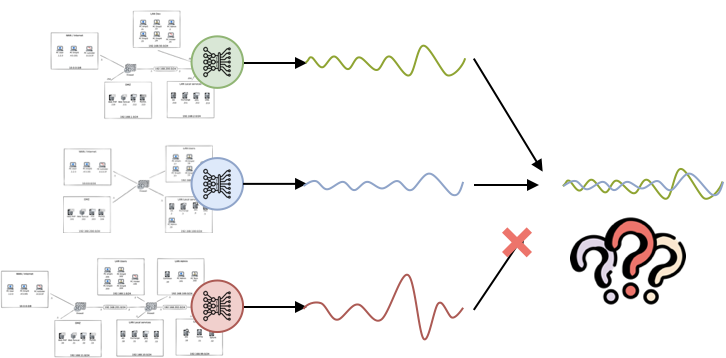
\includegraphics[width=\linewidth]{figures/intro/heterogeneity.png}
    \end{column}

    \begin{column}{.5\textwidth}

      \textcolor<2->{lightgray}{%
      \textbf{Challenge I}: \textit{Too much heterogeneity leads to poor performance\dots}
      }
      \only<1>{%
        \begin{itemize} \small
          \item How to handle different feature sets, data distributions?
          \item How to consider models that are dissimilar because they "contain" relevant knowledge?
        \end{itemize}
      }
      \vspace{1ex}


      \textcolor<1,3>{lightgray}{%
      \textbf{Challenge II}: \textit{Difficult to identify malicious contributions when models are different\dots}
      }
      
      \only<2>{%
        \begin{itemize} \small
          \item Are model "dissimilar" because they are different, or because they are malicious/poisoned?
        \end{itemize}
      }
      \vspace{1ex}
      
    \end{column}
  \end{columns}  
\end{frame}

\begin{frame}{Problem Statement}
  \begin{block}{Quality Assessment in Heterogeneous Settings}
    For $n$ participants $p_i$ and their local datasets $d_i$ of unknown similarity, each participant uploads a model update $w_i^r$ at each round $r$. Given $P = \{ p_1, p_2, \dots, p_n \} $ and $W = \{ w_1^r, w_2^r, \dots, w_n^r \} $, how can one assess the quality of each participant’s contribution without making assumptions on the data distribution across the datasets $d_i$?
  \end{block}
\end{frame}

\begin{frame}{Outline}
  \centering
  \begin{minipage}[t]{.8\textwidth}
    \tableofcontents%[hideallsubsections,]
  \end{minipage}
\end{frame}

% Architecture
% -----------------------------

\section{Architecture}

\subsection{Assessing Contribution Quality}

\begin{frame}{Existing Solutions}

  \begin{columns}[T]
    
    \begin{column}{.33\textwidth}
      \small\centering
      \textbf{Server-side evaluation}~\autocite{zhou_DifferentiallyPrivateFederated_2022}

      \begin{figure}
        \centering
        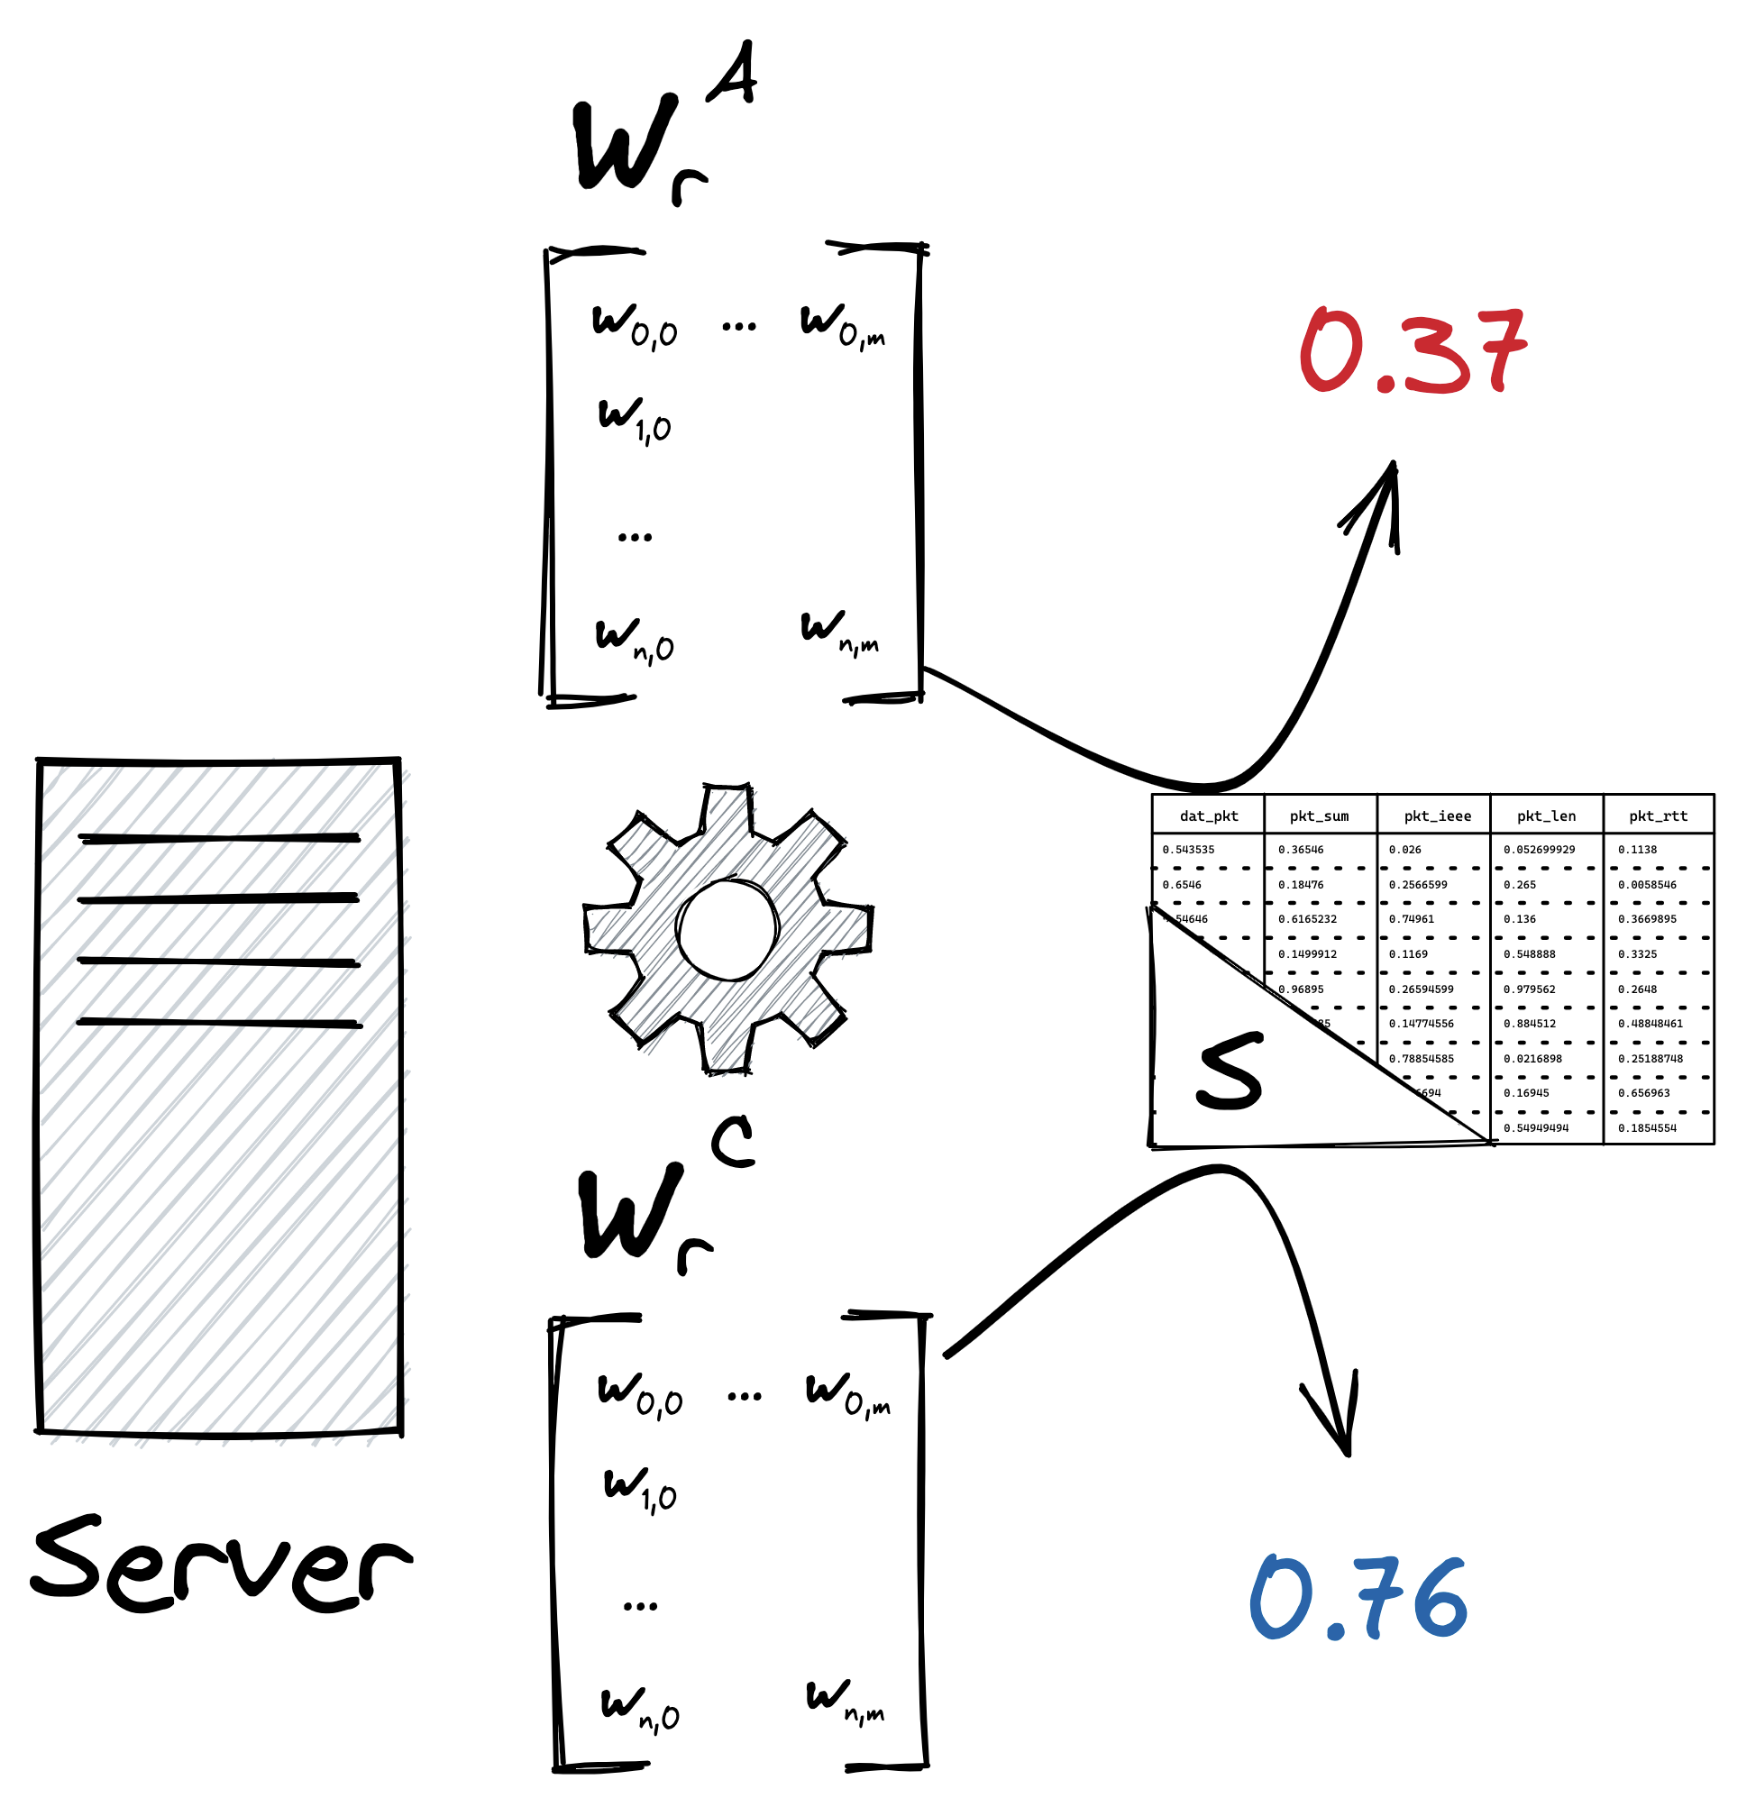
\includegraphics[height=.36\textheight]{figures/radar/server-side-eval}
      \end{figure}

      \begin{itemize}\smaller
        \item Only applicable in IID settings.
        \item Single source of truth.
      \end{itemize}
    \end{column}

    \onslide<2->{%
      \begin{column}{.33\textwidth}
        \small\centering
        \textbf{Server-side comparison}~\autocite{briggs_Federatedlearninghierarchical_2020}

        \begin{figure}
          \centering
          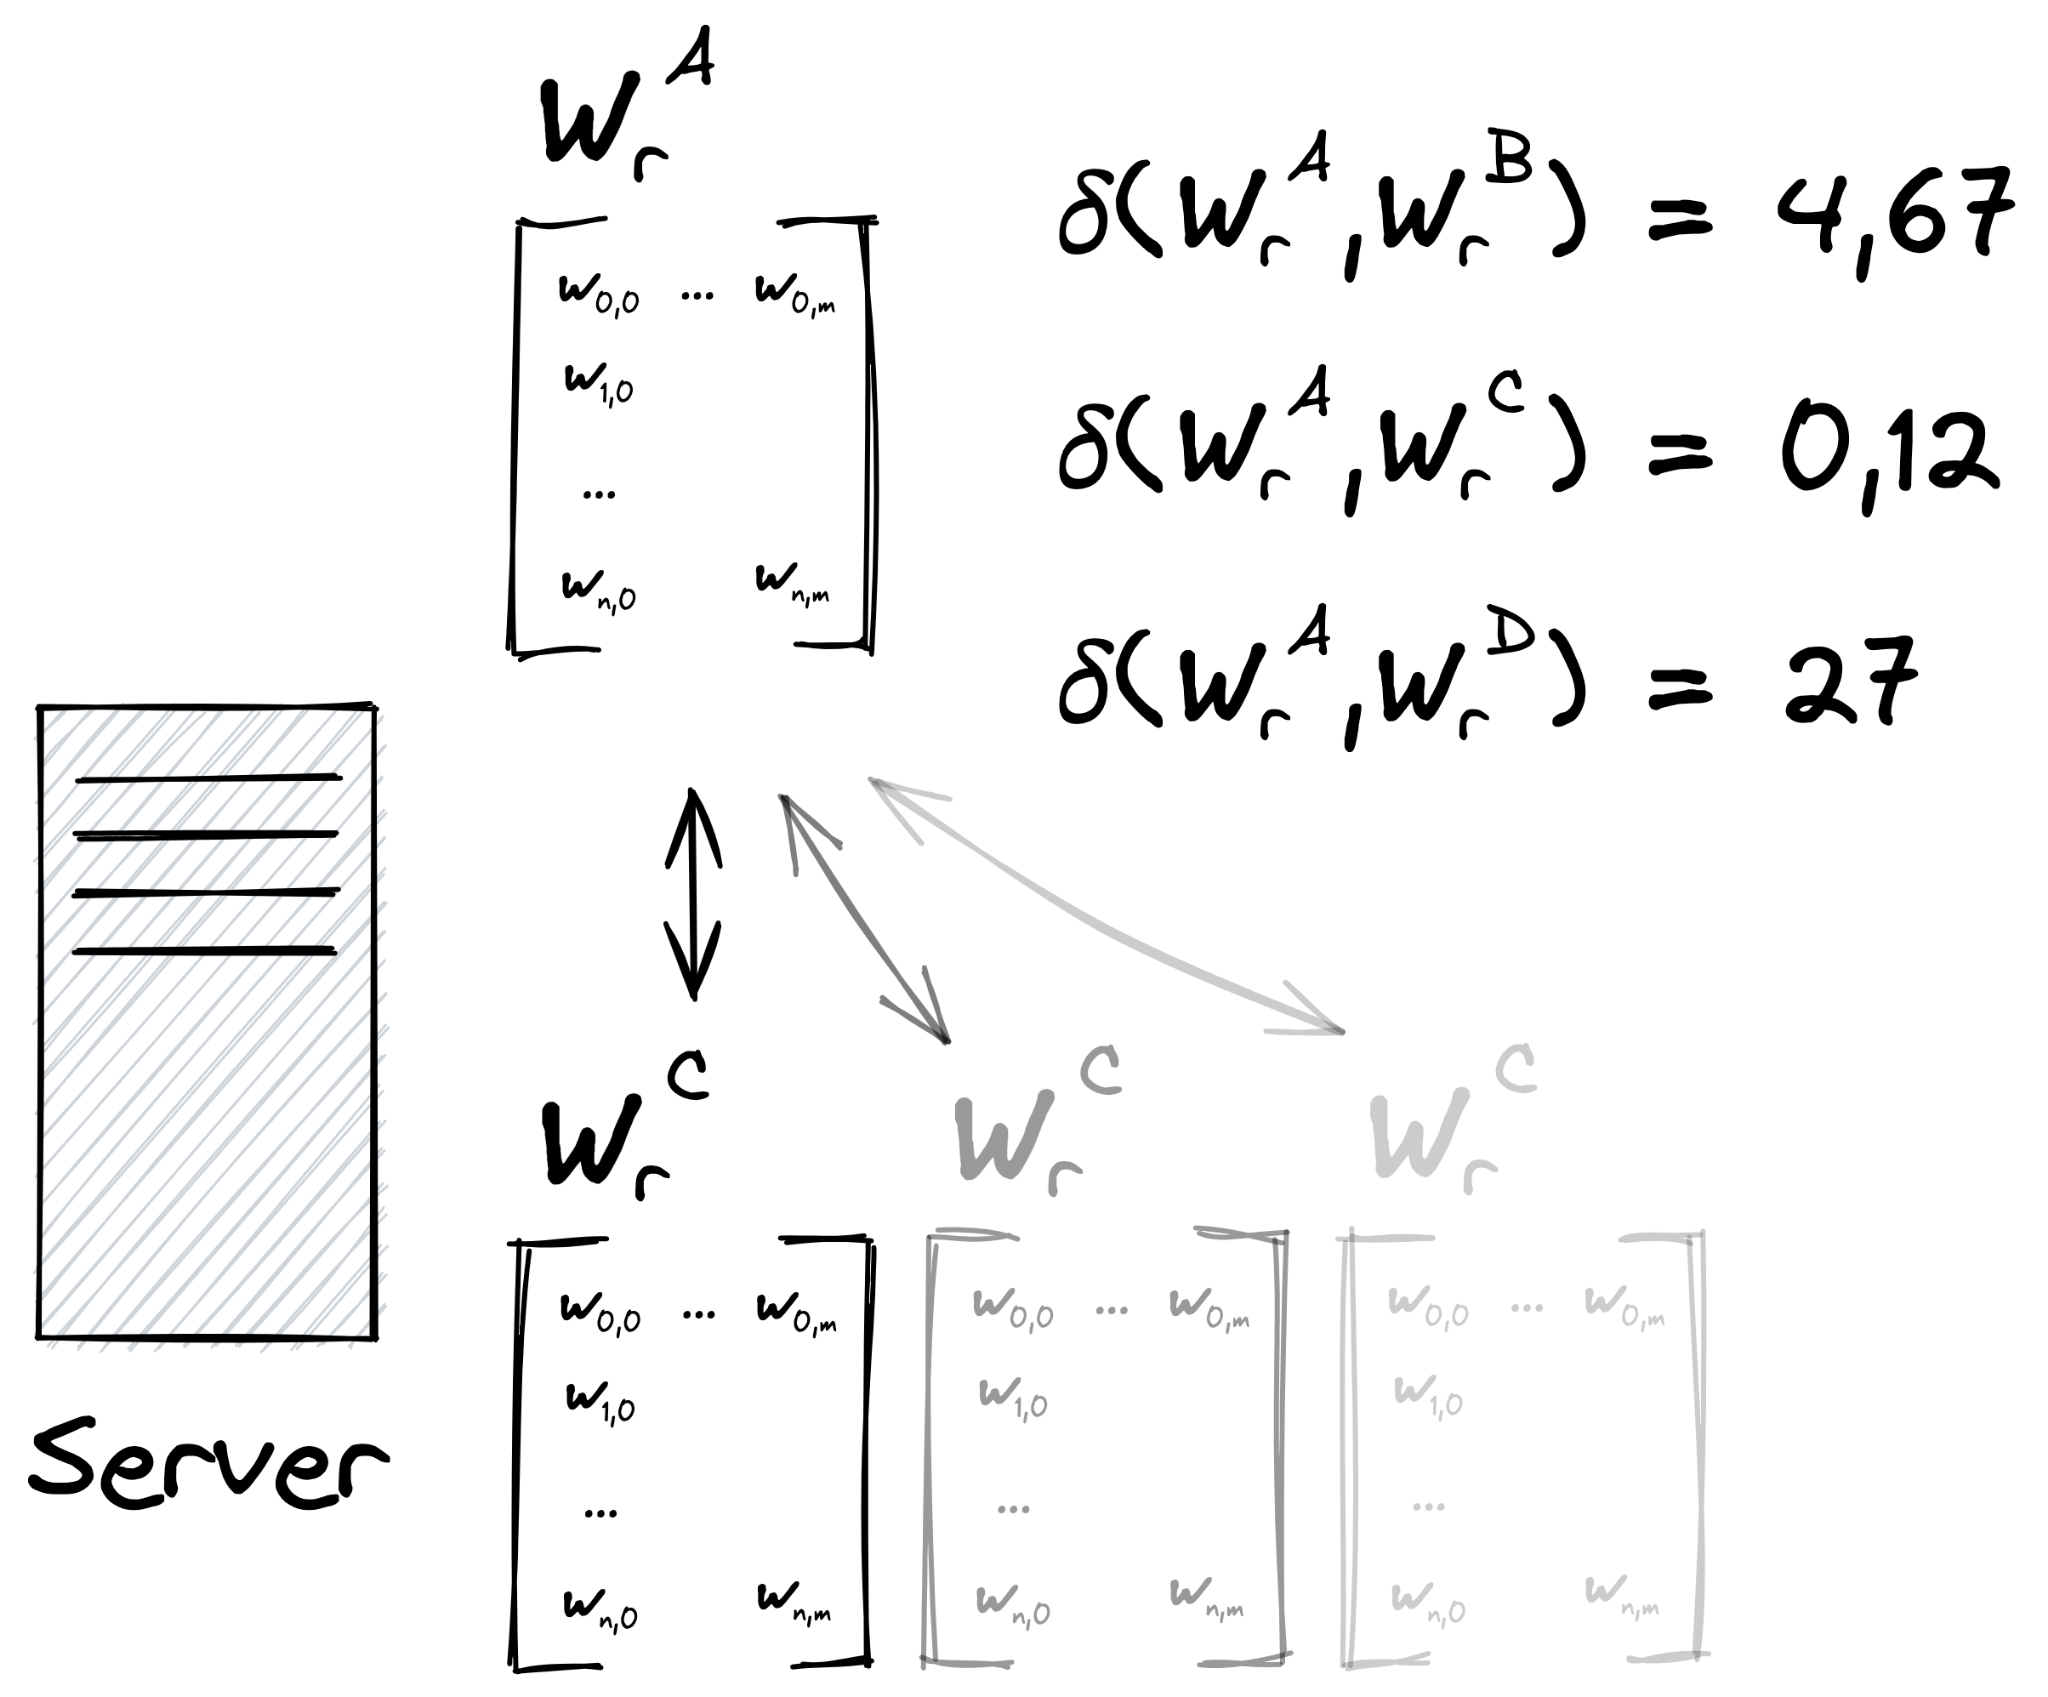
\includegraphics[height=.36\textheight]{figures/radar/server-side-comp}
        \end{figure}

        \begin{itemize}\smaller
          \item Less related to client data.
          \item More appropriate for high-dimensional data.
        \end{itemize}
      \end{column}%
    }

    \onslide<3->{%
      \begin{column}{.33\textwidth}
        \small\centering
        \textbf{Client-side evaluation}~\autocite{zhao_ShieldingCollaborativeLearning_2020}

        \begin{figure}
          \centering
          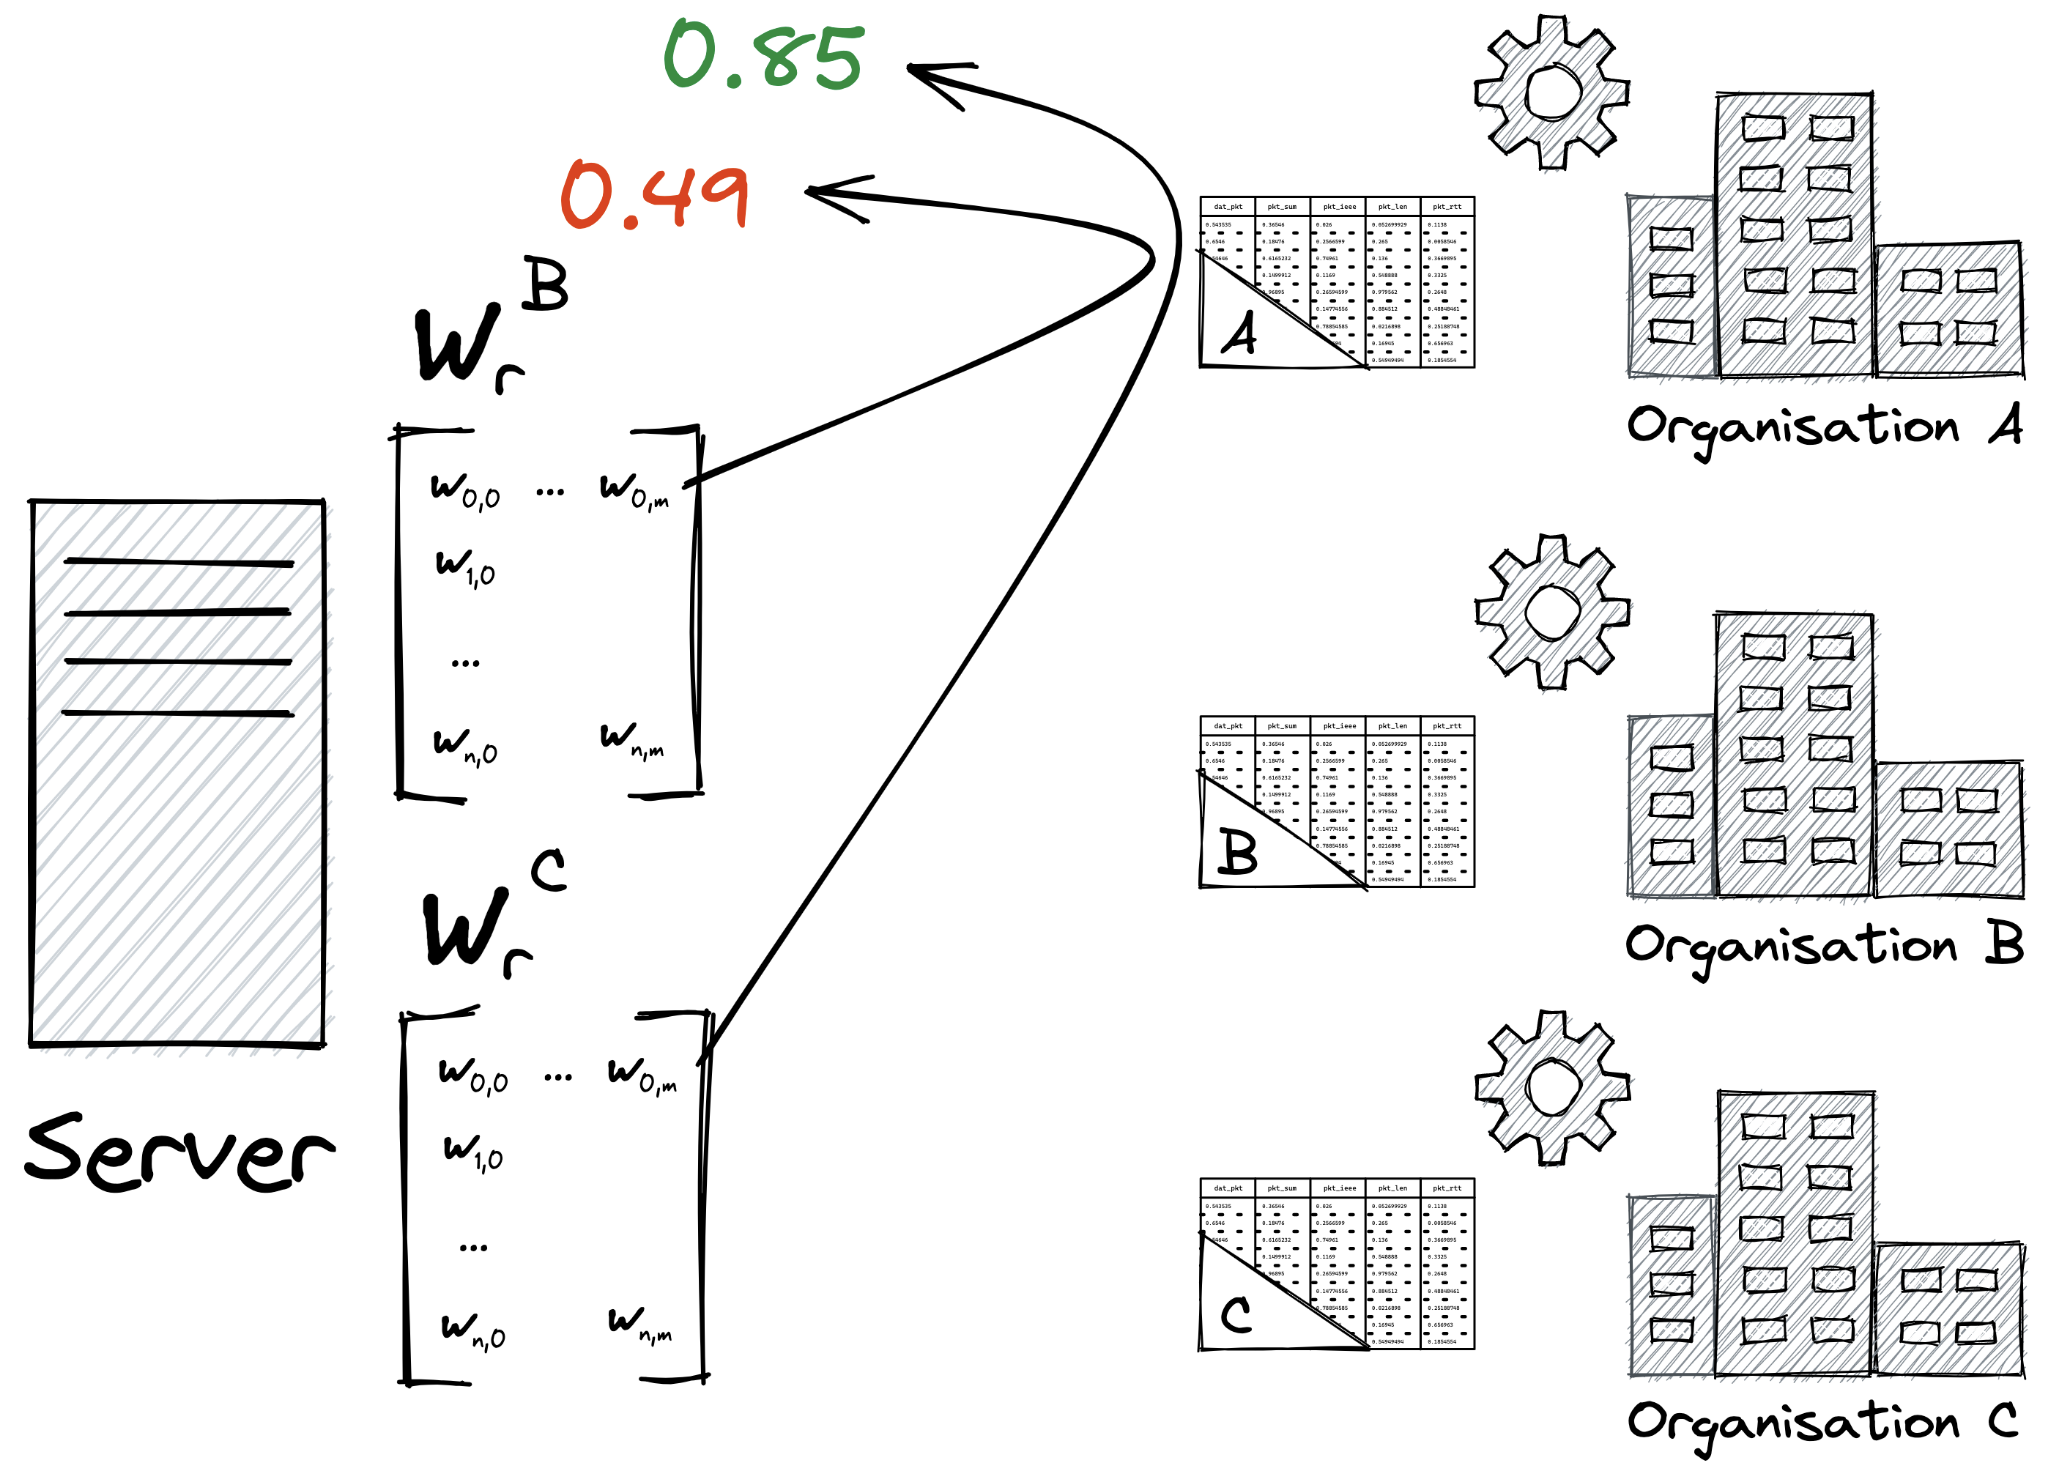
\includegraphics[height=.36\textheight]{figures/radar/client-side-eval}
        \end{figure}

        \begin{itemize}\smaller
          \item High cost in cross-device.
          \item More susceptible to badmouthing.
        \end{itemize}
      \end{column}%
    }

  \end{columns}

  \vspace{3ex}
  
  \fcitefootnote{zhou_DifferentiallyPrivateFederated_2022}
  \only<2->{\fcitefootnote{briggs_Federatedlearninghierarchical_2020}}
  \only<3->{\fcitefootnote{zhao_ShieldingCollaborativeLearning_2020}}

\end{frame}

\begin{frame}{Assessing Quality with Cross-Evaluation}

  \begin{columns}
    \begin{column}{.45\textwidth}
      \begin{figure}
        \centering
        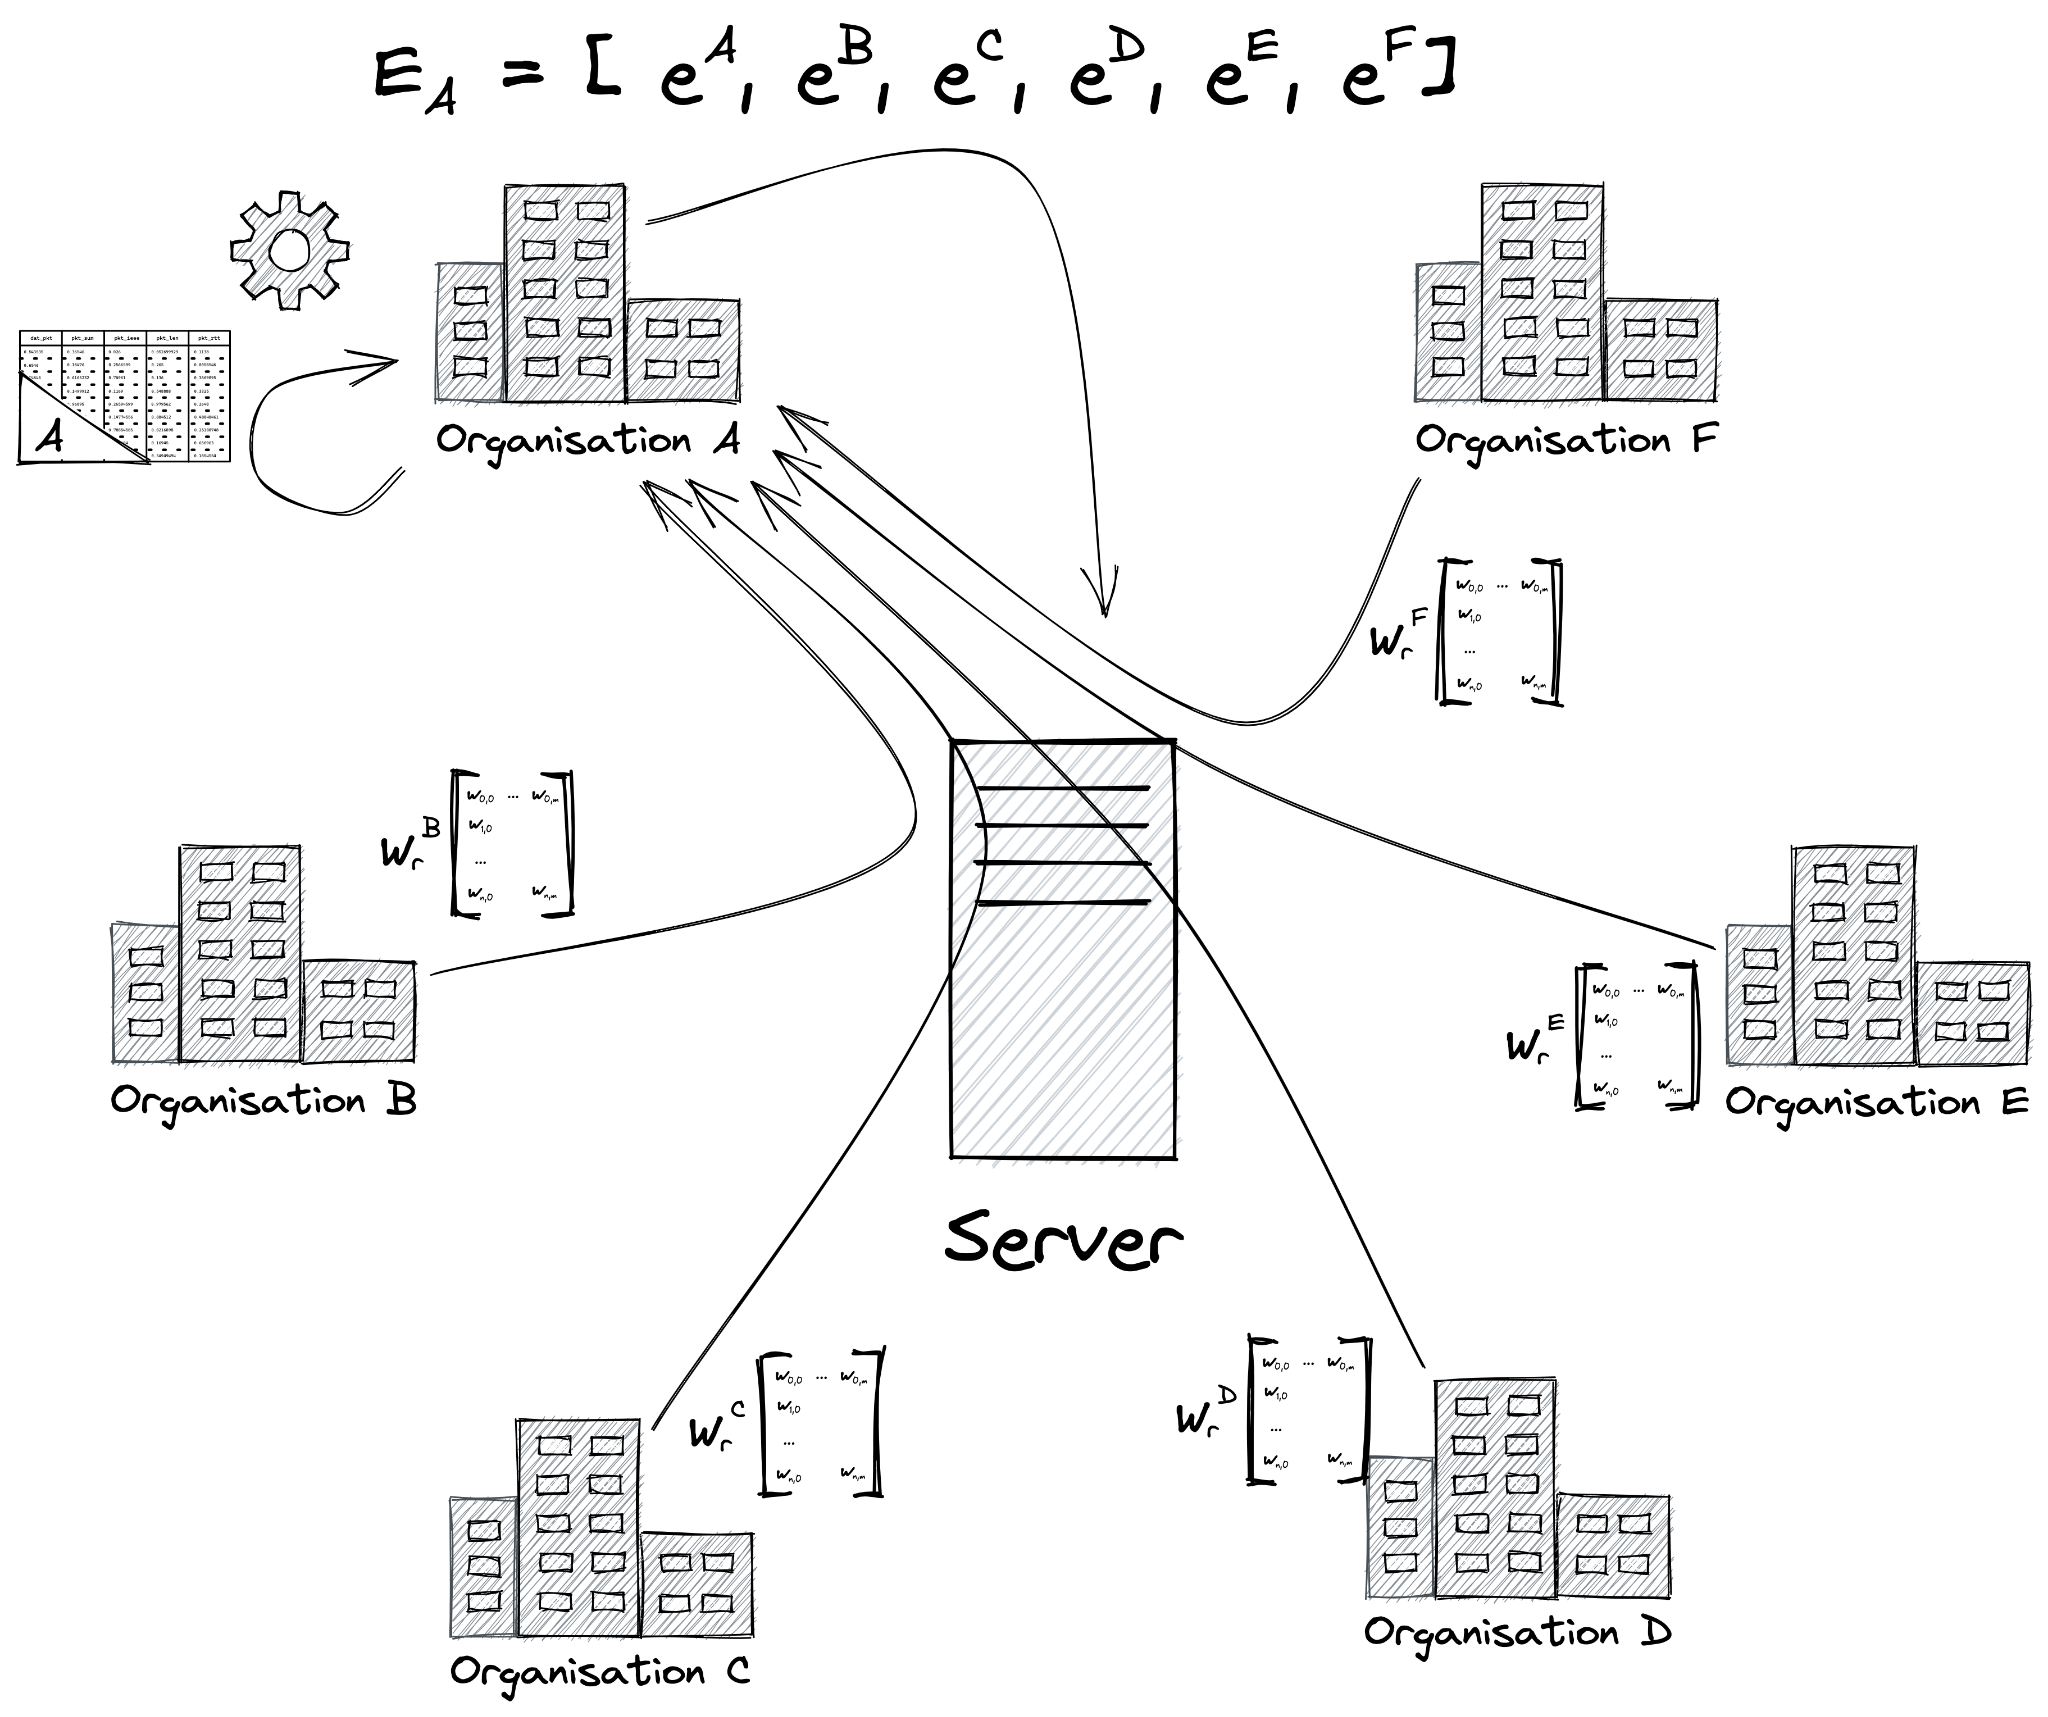
\includegraphics[width=\textwidth]{figures/radar/xeval}
      \end{figure}
    \end{column}
    
    \begin{column}{.55\textwidth}
      \small
      \setlength{\baselineskip}{0.8\baselineskip}
      \vspace{1ex}

      \textbf{Advantages}
      \begin{itemize}
        \item The central server does not need prior knowledge.
        \item Evaluates how each model fits the data (\eg, accuracy, F1 score).
        \item Exhaustive overview of the entire system at each round $r$.
      \end{itemize}

      \onslide<2->{%
        \textbf{Drawbacks}
        \begin{itemize}
          \item High communication and computation costs.
          \item Does not scale well.
          \item Shares local models to participants: less privacy-friendly.
        \end{itemize}
      }

      \onslide<3->{%
        \textbf{But\dots}
        \begin{itemize}
          \item Cross-silo use case: few clients, with reasonable computing capacity.
          \item Slow workflow: long time between rounds.
        \end{itemize}
      }   
    \end{column}

  \end{columns}

\end{frame}

\subsection{Fighting Heterogeneity with Clustering}

\begin{frame}{Fighting Heterogeneity with Clustering}
  \begin{columns}
    \begin{column}{.55\textwidth}
      \textbf{Objective}
      \begin{itemize}
        \item Reduce heterogeneity for the aggregation.
        \item Build communities of \emph{more} homogeneous participants.
      \end{itemize}


      \onslide<2>{%
        \textbf{Clustering for FL}
        \begin{itemize}
          \item Regarding data-source:
          \begin{itemize}
            \item Gradient/model similarity.~\autocite{briggs_Federatedlearninghierarchical_2020}
            \item Cross-evaluation results.
          \end{itemize}

          \item Clustering methods:
          \begin{itemize}
            \item Dynamic \emph{split-and-merge}.~\autocite{chen_ZeroKnowledgeClustering_2021}
            \item Hierarchical clustering.~\autocite{briggs_Federatedlearninghierarchical_2020}
          \end{itemize}
        \end{itemize}
      }
      
    \end{column}
    \begin{column}{.45\textwidth}
      \begin{figure}
        \centering
        \makebox[\textwidth][c]{%
          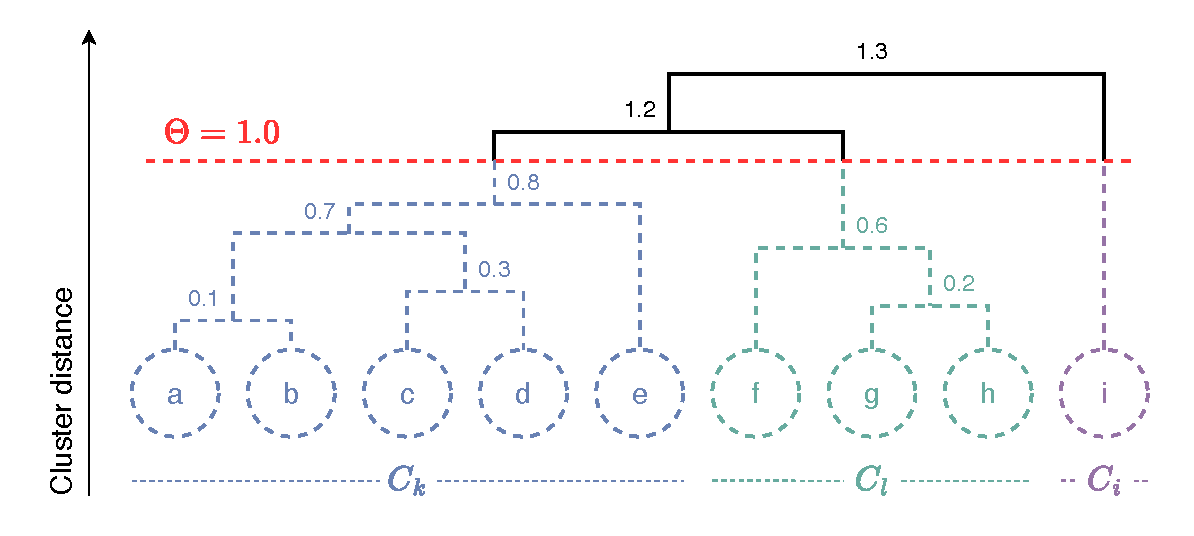
\includegraphics[width=1.2\textwidth]{figures/radar/clustering.drawio.pdf}%
        }
        %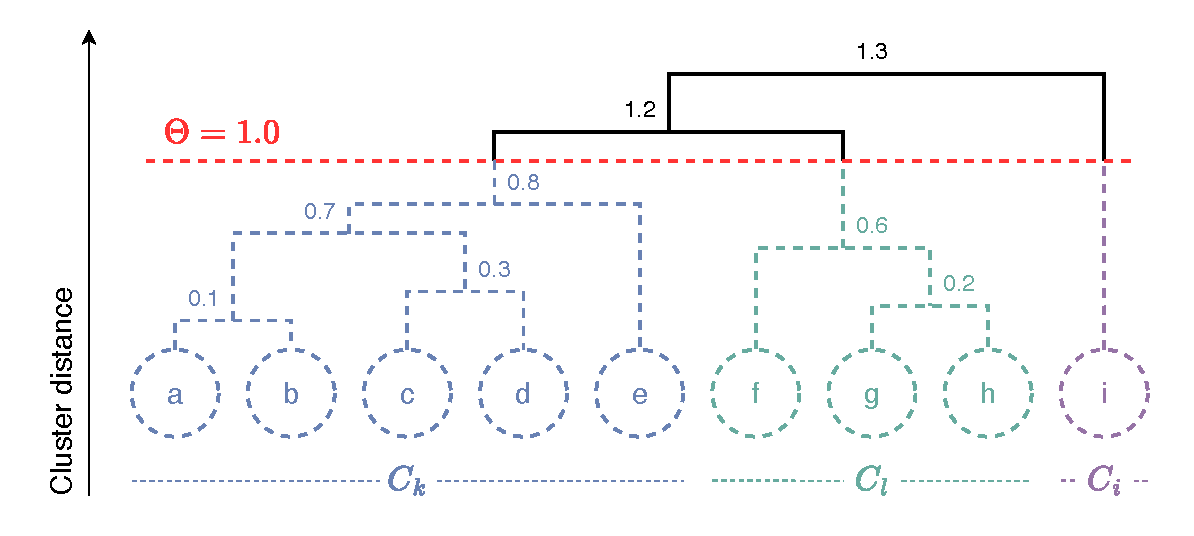
\includegraphics[width=\textwidth]{figures/radar/clustering.drawio.pdf}
        \caption{Hierarchical clustering.}
      \end{figure}
    \end{column}
  \end{columns}
  

  \only<2>{%
    \fcitefootnote{briggs_Federatedlearninghierarchical_2020}
    \fcitefootnote{chen_ZeroKnowledgeClustering_2021}
  }

\end{frame}

\subsection{Mitigating Byzantine Contributions}

\begin{frame}{Reputation-aware Aggregation}

  \begin{block}{Definition: Reputation Systems\normalfont~\autocite{resnick_Reputationsystems_2000}}
    \begin{itemize}
      \item Long-lived entities that inspire an expectation of future interaction;
      \item Capture and distribution of feedback about current interactions (such information must be visible in the future); and
      \item Use of feedback to guide trust decisions.
    \end{itemize}
  \end{block}

  \onslide<2>{%
    \begin{itemize}
      \item Dirichlet distribution for local aggregation of the reputation scores.~\autocite{fung_DirichletBasedTrustManagement_2011}
      \item Votes weighted by the similarity inside each cluster.
      \item Exponential decay for potential redemption.
    \end{itemize}
  }

  \fcitefootnote{resnick_Reputationsystems_2000}
  \only<2>{%
    \fcitefootnote{fung_DirichletBasedTrustManagement_2011}
  }

\end{frame}

% Evaluation Setup
% -----------------------------

\section{Evaluation Setup}

\begin{frame}{Experimental Setup}
  \begin{columns}
    \begin{column}{.55\textwidth}
      Similar setup as in the previous case study:
      \begin{itemize}
        \item Heterogeneous datasets, but some participants can share similarities.
        \item 4 datasets: CIC-CSE-IDS2018, UNSW-NB15, Bot-IoT, ToN\_IoT.
        \item NF-V2~\autocite{sarhan_StandardFeatureSet_2021} feature set (\ie, NetFlow V9).
      \end{itemize}
    \end{column}
    \begin{column}{.45\textwidth}
      \begin{figure}

        \includegraphics<1>[height=.5\textheight,left]{figures/radar/distribution.png}%
        \includegraphics<2>[height=.5\textheight,left]{figures/radar/distribution-attack.png}%

        \caption{Distribution of the datasets.}
      \end{figure}
    \end{column}
  \end{columns}
  \fcitefootnote{sarhan_StandardFeatureSet_2021}
\end{frame}


% Results
% -----------------------------

\section{Results}

\begin{frame}{Results}
  \begin{table}
    \centering
    \caption{
      \emph{Effect of different attack configurations (untargeted) on all baselines.}
      \texttt{RA} is RADAR, \texttt{FG} is \texttt{FoolsGold}, \texttt{FA} is \texttt{FedAvg} (on \emph{all} participants), and \texttt{FC} is \texttt{FedAvg} ideally clustered per dataset.
    }

    \footnotesize

    \newcommand{\hl}{}
    \only<2>{\renewcommand{\hl}{\cellcolor{imta-green!30}}}


  
    \setlength\tabcolsep{1ex}
    \begin{tabularx}{.8\textwidth}{lX|rrrr|rrrr}
      \toprule % ---------------------------------
      \multicolumn{2}{c|}{\multirow{2}{*}{\textbf{Scenario}}} & \multicolumn{4}{c|}{\textbf{Mean accuracy} (\%)} & \multicolumn{4}{c}{\textbf{\gls{asr}} (\%)} \\
      & & \multicolumn{1}{c}{\texttt{RA}} & \multicolumn{1}{c}{\texttt{FG}} & \multicolumn{1}{c}{\texttt{FA}} & \multicolumn{1}{c|}{\texttt{FC}} & \multicolumn{1}{c}{\texttt{RA}} & \multicolumn{1}{c}{\texttt{FG}} & \multicolumn{1}{c}{\texttt{FA}} & \multicolumn{1}{c}{\texttt{FC}} \\
      \midrule % ---------------------------------
      % TARGETED ATTACKS
      \multicolumn{2}{l|}{\textbf{Targeted} (\texttt{100T})} & & & & & & & & \\
                  & \texttt{Benign}       & \hl 99.07 & 55.04 & 79.49 & \textbf{99.24} & \hl \textbf{0.00} &  5.17 & 5.10 &  0.09 \\
                  & \texttt{Lone}         & \hl 99.06 & 60.51 & 77.38 & \textbf{99.22} & \hl \textbf{0.00} & 93.82 & 6.73 &  0.45 \\
                  & \texttt{Collud. min.} & \hl \textbf{98.96} & 54.64 & 78.48 & 98.33 & \hl \textbf{0.00} &  2.97 & 9.99 & 53.40 \\
                  & \texttt{Collud. maj.} & \hl \textbf{98.28} & 85.10 & 79.40 & 98.22 & \hl \only<3>{\bfseries\color{red}} 73.39 & \textbf{8.10} & 17.65 & 59.36 \\
      \midrule % ---------------------------------
      % UNTARGETED ATTACKS
      \multicolumn{2}{l|}{\textbf{Untargeted} (\texttt{100U})} & & & & & & & & \\
      & \texttt{Benign}        & \hl 99.07 & 55.04 & 79.49 & \textbf{99.24} & \hl 0.09  & 0.39 & 33.30 & \textbf{0.06} \\
      & \texttt{Lone}          & \hl 98.96 & 49.56 & 78.38 & \textbf{99.22} &\hl \textbf{0.08} & 99.89 & 54.70 & 0.12 \\
      & \texttt{Collud. min.}  & \hl \textbf{98.98} & 49.67 & 72.47 & 97.69 & \hl 0.10 & \textbf{0.04} & 44.53 & 6.26 \\
      & \texttt{Collud. maj.}  & \hl \textbf{98.96} & 69.09 & 81.87 & 75.66 & \hl \textbf{0.08} & 38.98 & 59.49 & 94.36 \\          
      \bottomrule % ---------------------------------
      \small & \multicolumn{1}{c}{} & \multicolumn{4}{c}{\emph{higher is better}} & \multicolumn{4}{c}{\emph{lower is better}}
    \end{tabularx}
  \end{table}
  
\end{frame}


% Conclusion
% -----------------------------

\section*{Conclusion}

\begin{frame}
  \sectionpage
\end{frame}

\begin{frame}{Fighting Byzantine Attacks in Federated Learning}
  \textbf{The proposed framework can:}
  \begin{itemize}
    \item Accurately cluster similar participants based on cross evaluations results.
    \item Mitigate label-flipping untargeted attacks via clustering.
    \item Mitigate most label-flipping targeted attacks, including colluding attackers (up to 80\% of poisoned data).
  \end{itemize}

  \pause
  \textbf{How generic?}
  \begin{itemize}
    \item Only few conditions: parametric models, locally owned evaluation set, a \alert<3>{small-scale use case}, and a \alert<3>{trusted central server}.
  \end{itemize}
\end{frame}


\begin{frame}{Future Work}
  \textbf{Future works:}
    \begin{itemize}
      \item Remove the central server dependency.
      \item Reduce the cross-evaluation overhead to extend applicability to cross device settings.
      \item Test the approach in more realistic heterogeneous settings.
    \end{itemize}
\end{frame}


\begin{frame}
  \centering\scshape\large Thank you for your attention!

  \vfill
  
  \normalshape\normalsize

  \textbf{RADAR: Model Quality Assessment for Reputation-aware Collaborative Federated Learning}
  \medskip
  \raggedright
  \begin{itemize}
    \item blah
    \item blah
    \item \dots
  \end{itemize}

  \vfill

  \centering\small
  leo.lavaur@imt-atlantique.fr\\
  pierre-marie.lechevalier@imt-atlantique.fr

\end{frame}


\appendix

\begin{frame}[allowframebreaks]{References}
  \printbibliography[heading=none]
\end{frame}

% Backup Slides
% -----------------------------

\section*{Extra Slides}

\begin{frame}
  \sectionpage
\end{frame}

\begin{frame}{Intrusion Detection}
  
  \textbf{Machine Learning (ML) for Network-based Intrusion Detection Systems (NIDSs)}
  \begin{itemize}
    \item Detect \alert{malicious} activities (\ie, \textit{misuse detection}) or \alert{anomalies} (\ie, \textit{anomaly detection}).
    \item Various types of algorithms: \alert<2>{supervised}, unsupervised, semi-supervised, reinforcement learning, \textit{etc}.
    \item Great performance with Deep Learning (DL) (on public datasets at least).
  \end{itemize}
  \bigskip
    
  \begin{figure}
    \centering
    \makebox[\textwidth][c]{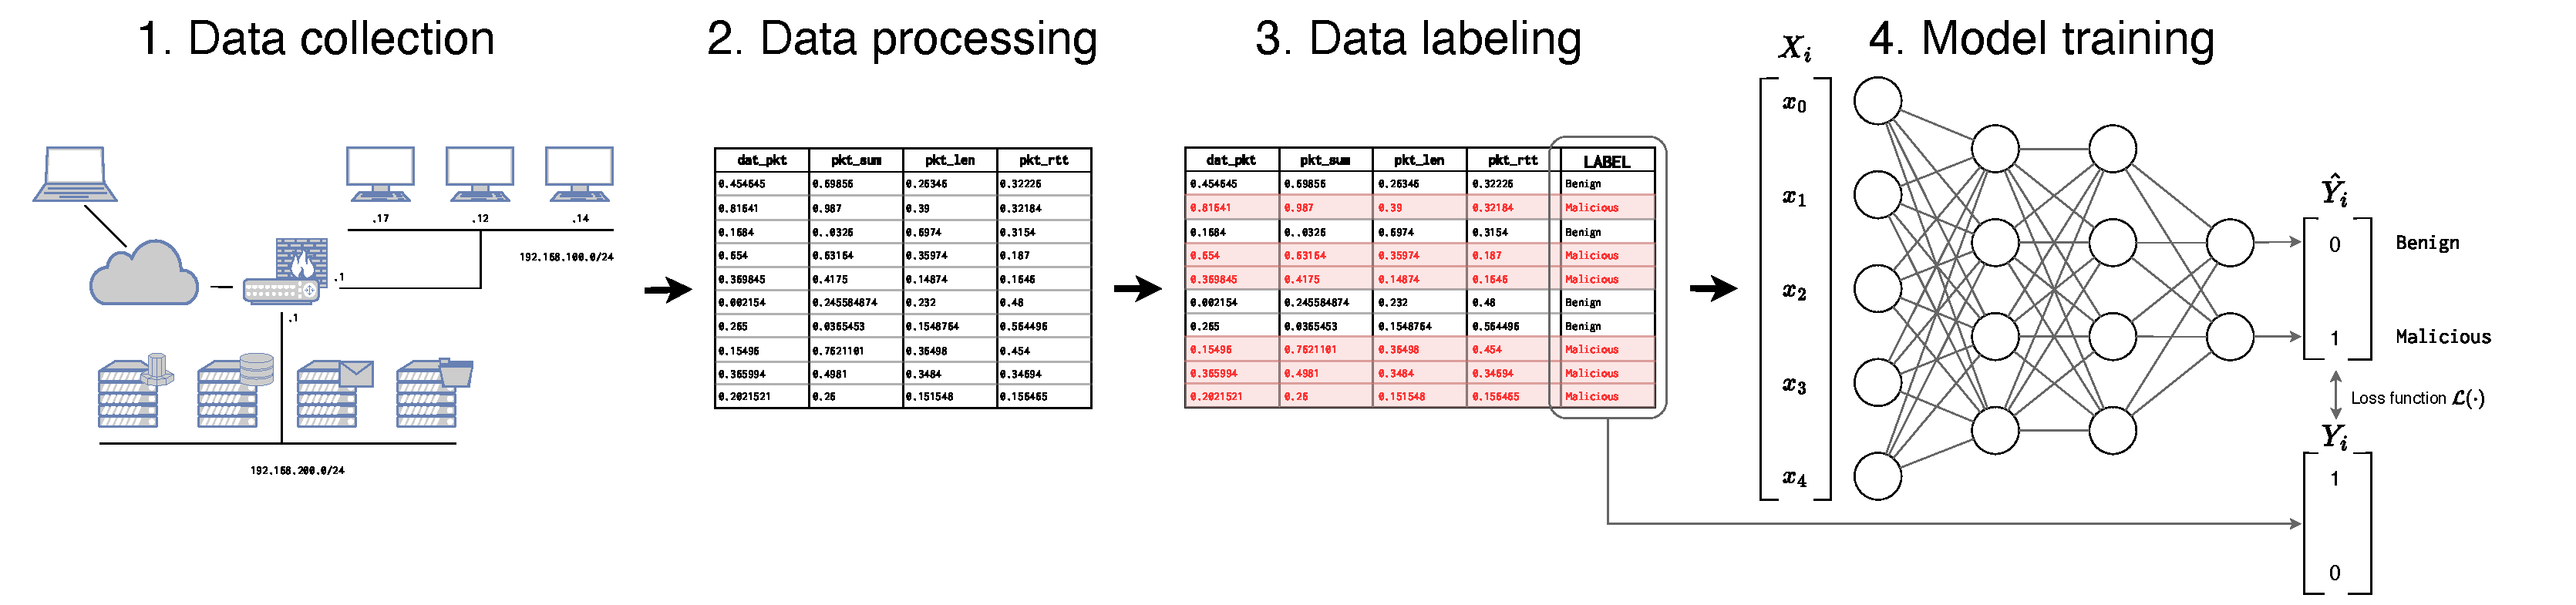
\includegraphics[width=.9\textwidth]{figures/intro/mlp-workflow.pdf}}
    \caption{Typical workflow for ML-based NIDSs.}
  \end{figure}
\end{frame}

\begin{frame}{Intrusion Detection}

  \begin{columns}
    \begin{column}{0.5\textwidth}
        \textbf{Challenges:}
        \begin{itemize}
          \item not enough labelled data;
          \item risk of local bias or skewed data distribution;
          \item inefficient against new attacks, especially \alert{supervised} approaches.
        \end{itemize}
    \end{column}

    \begin{column}{0.5\textwidth}
      \begin{figure}
        \centering
        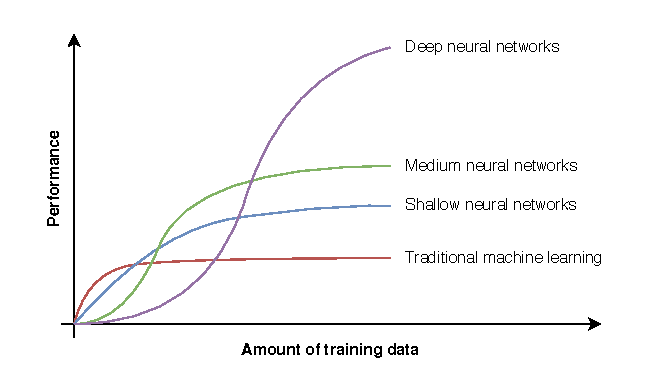
\includegraphics[width=\linewidth]{figures/intro/ml-perf}
      \end{figure}
    \end{column}
  \end{columns}
\end{frame}

\begin{frame}{Scaling Intrusion Detection}

  \textbf{Federated Learning (FL)}
  
  \begin{itemize}
    \item Novel-\emph{ish} distributed ML paradigm (Google, 2017)~\cite{mcmahan_Communicationefficientlearningdeep_2017}.
    \item Distributed clients can train a common model without sharing their training data.
    \item Privacy-preserving: high level of abstraction for the shared models preventing data leakage.
  \end{itemize}
\end{frame}

\begin{frame}{FL Fundamentals}
  \vspace{-1em}
  \begin{figure}
    \centering
    \only<1>{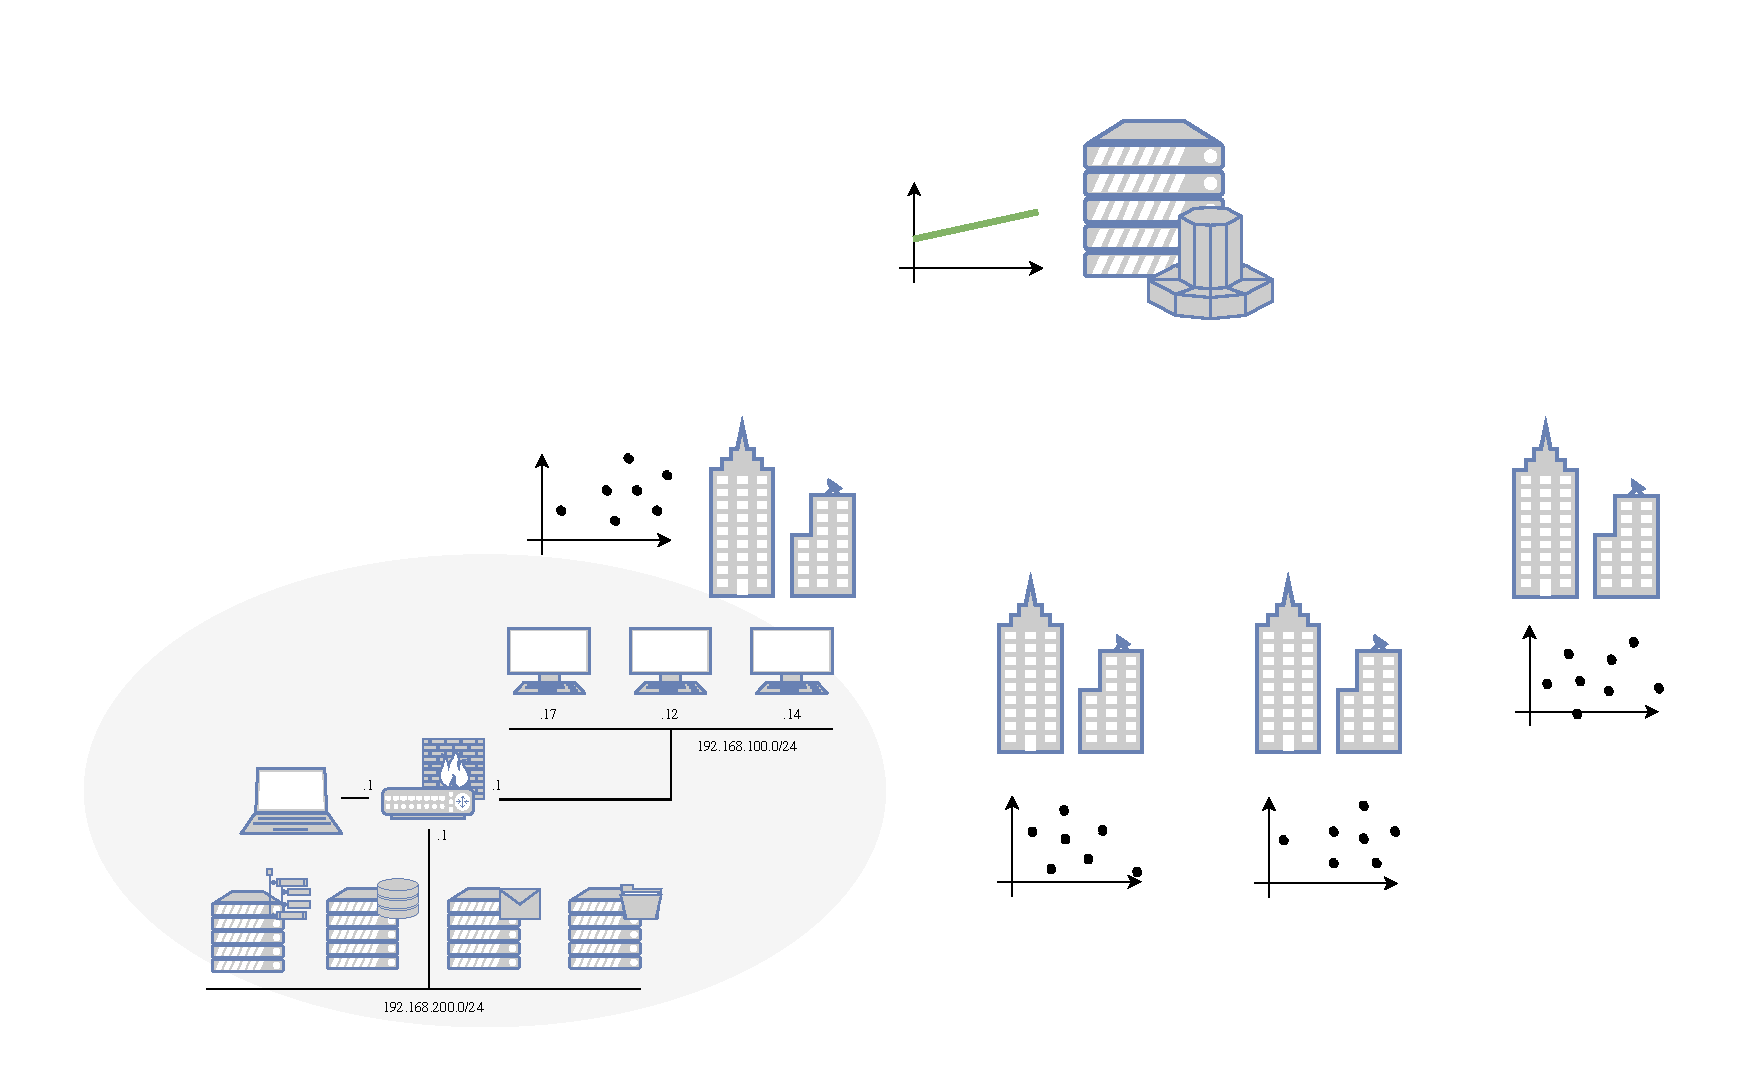
\includegraphics[width=.75\linewidth]{./figures/intro/fl/0.pdf}}%
    \only<2>{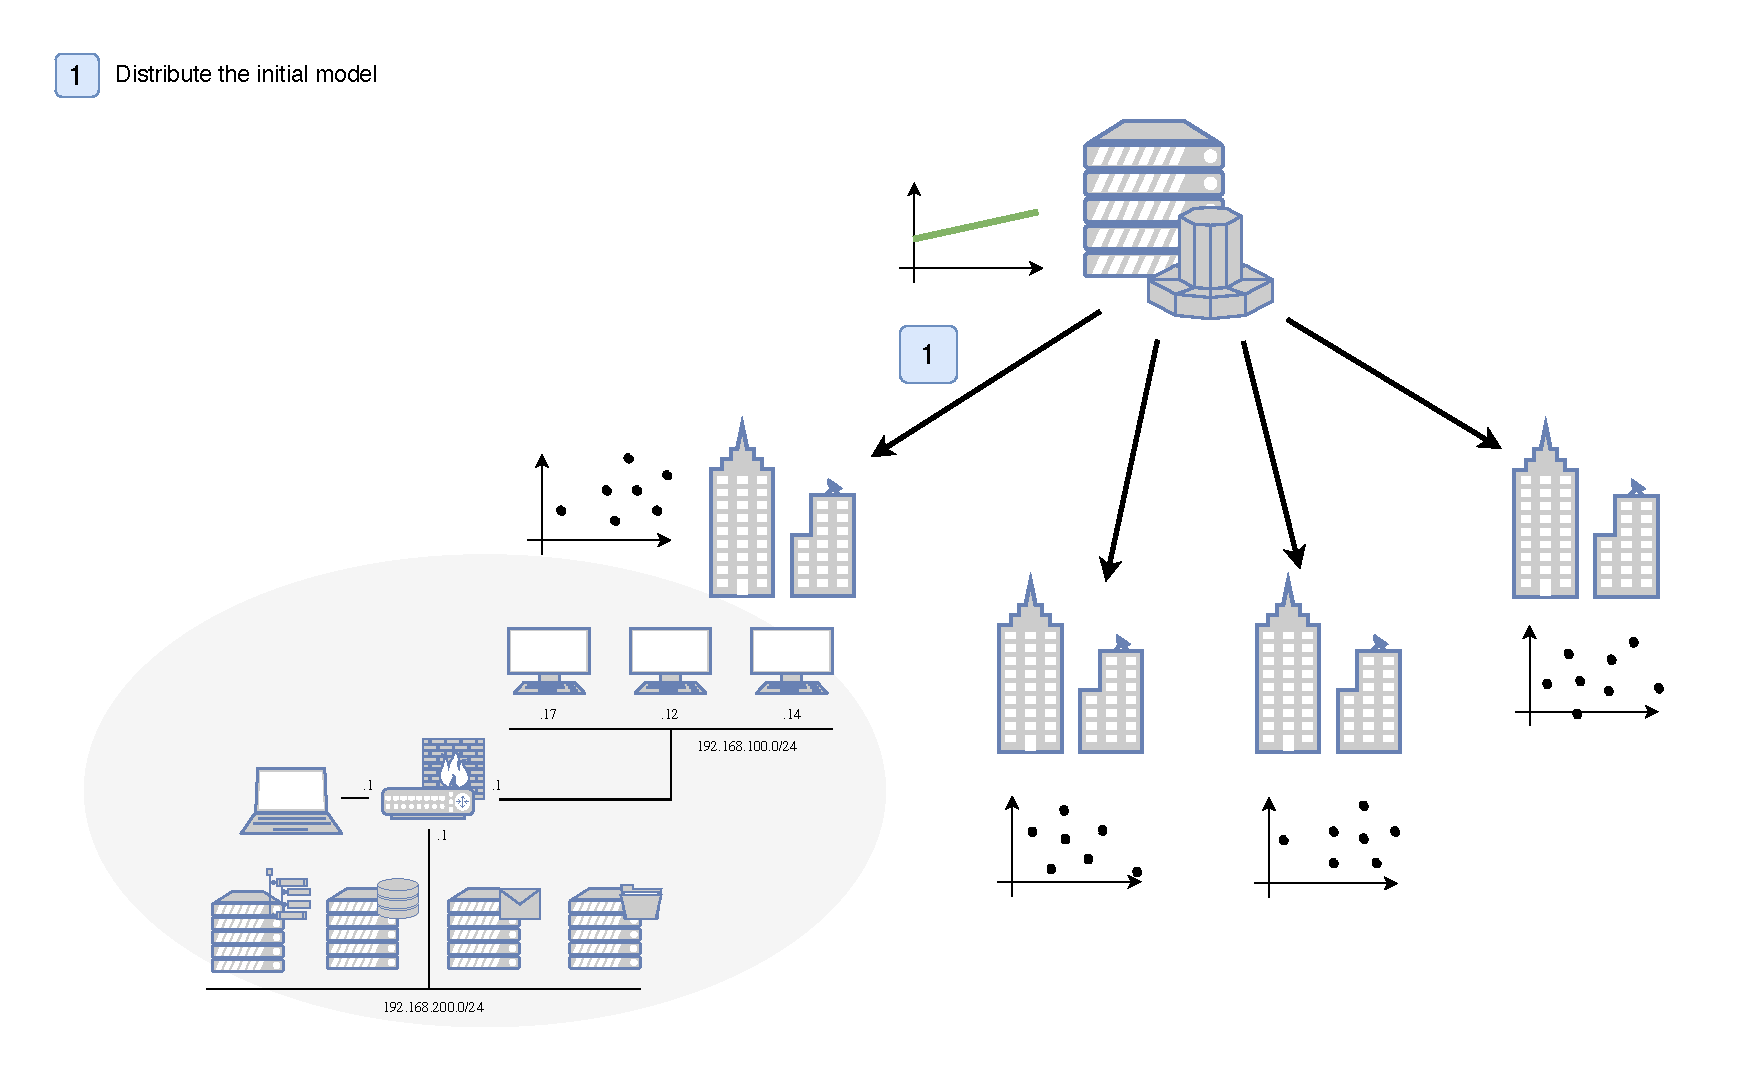
\includegraphics[width=.75\linewidth]{./figures/intro/fl/1.pdf}}%
    % Cannot use animations with MacOS Preview.
    % \only<3>{\animategraphics[width=.75\linewidth,loop,autoplay]{2}{./figures/intro/fl/2-}{1}{2}}%
    \only<3>{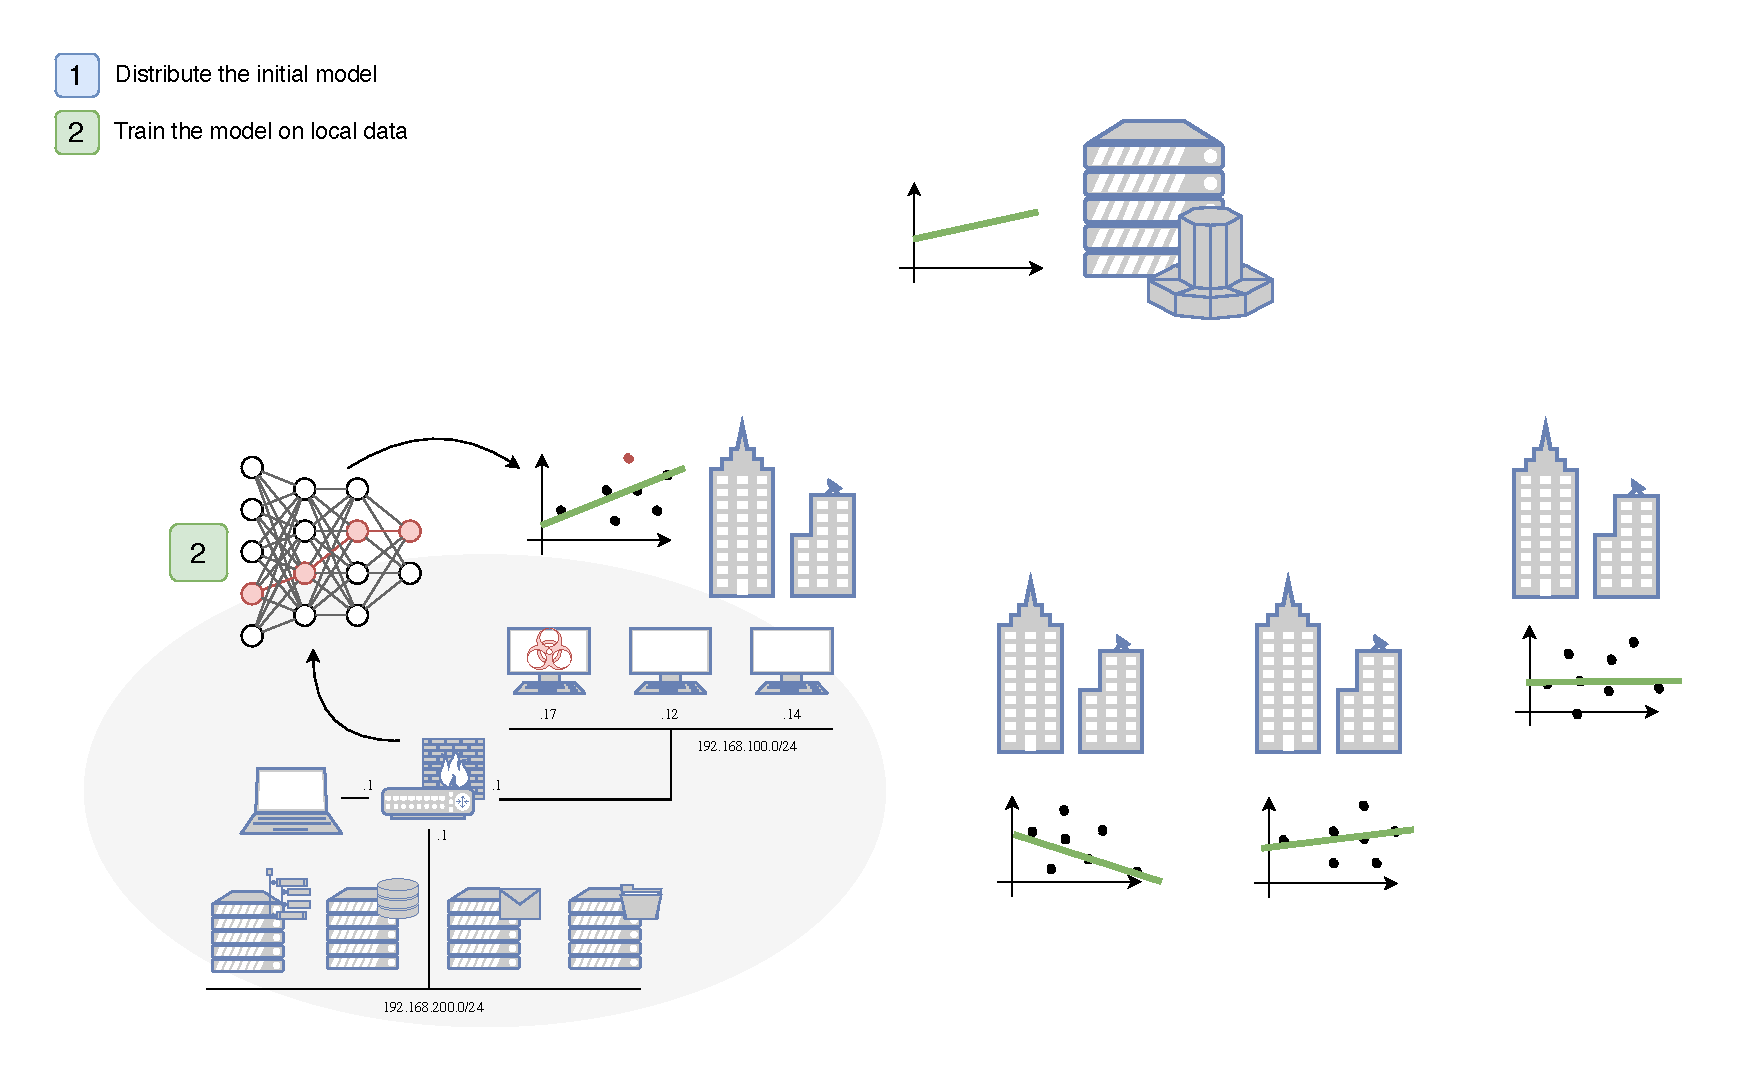
\includegraphics[width=.75\linewidth]{./figures/intro/fl/2-2.pdf}}%
    \only<4>{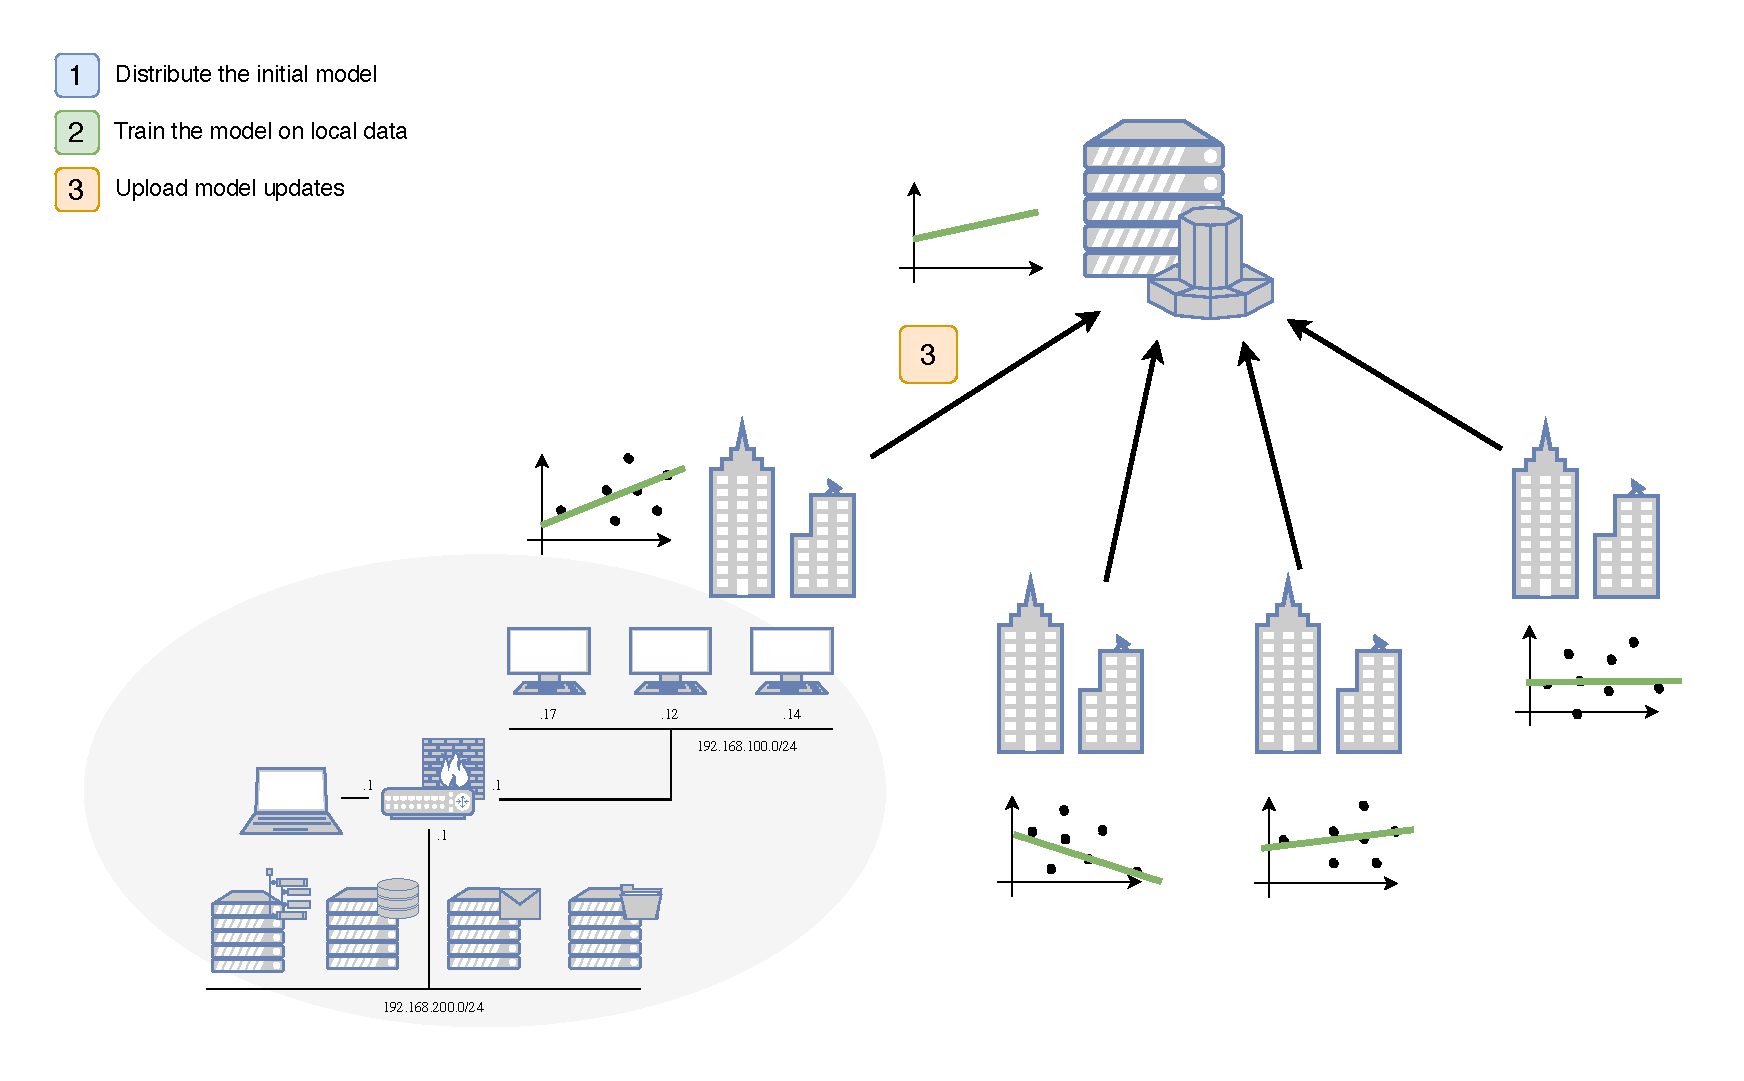
\includegraphics[width=.75\linewidth]{./figures/intro/fl/3.pdf}}%
    \only<5>{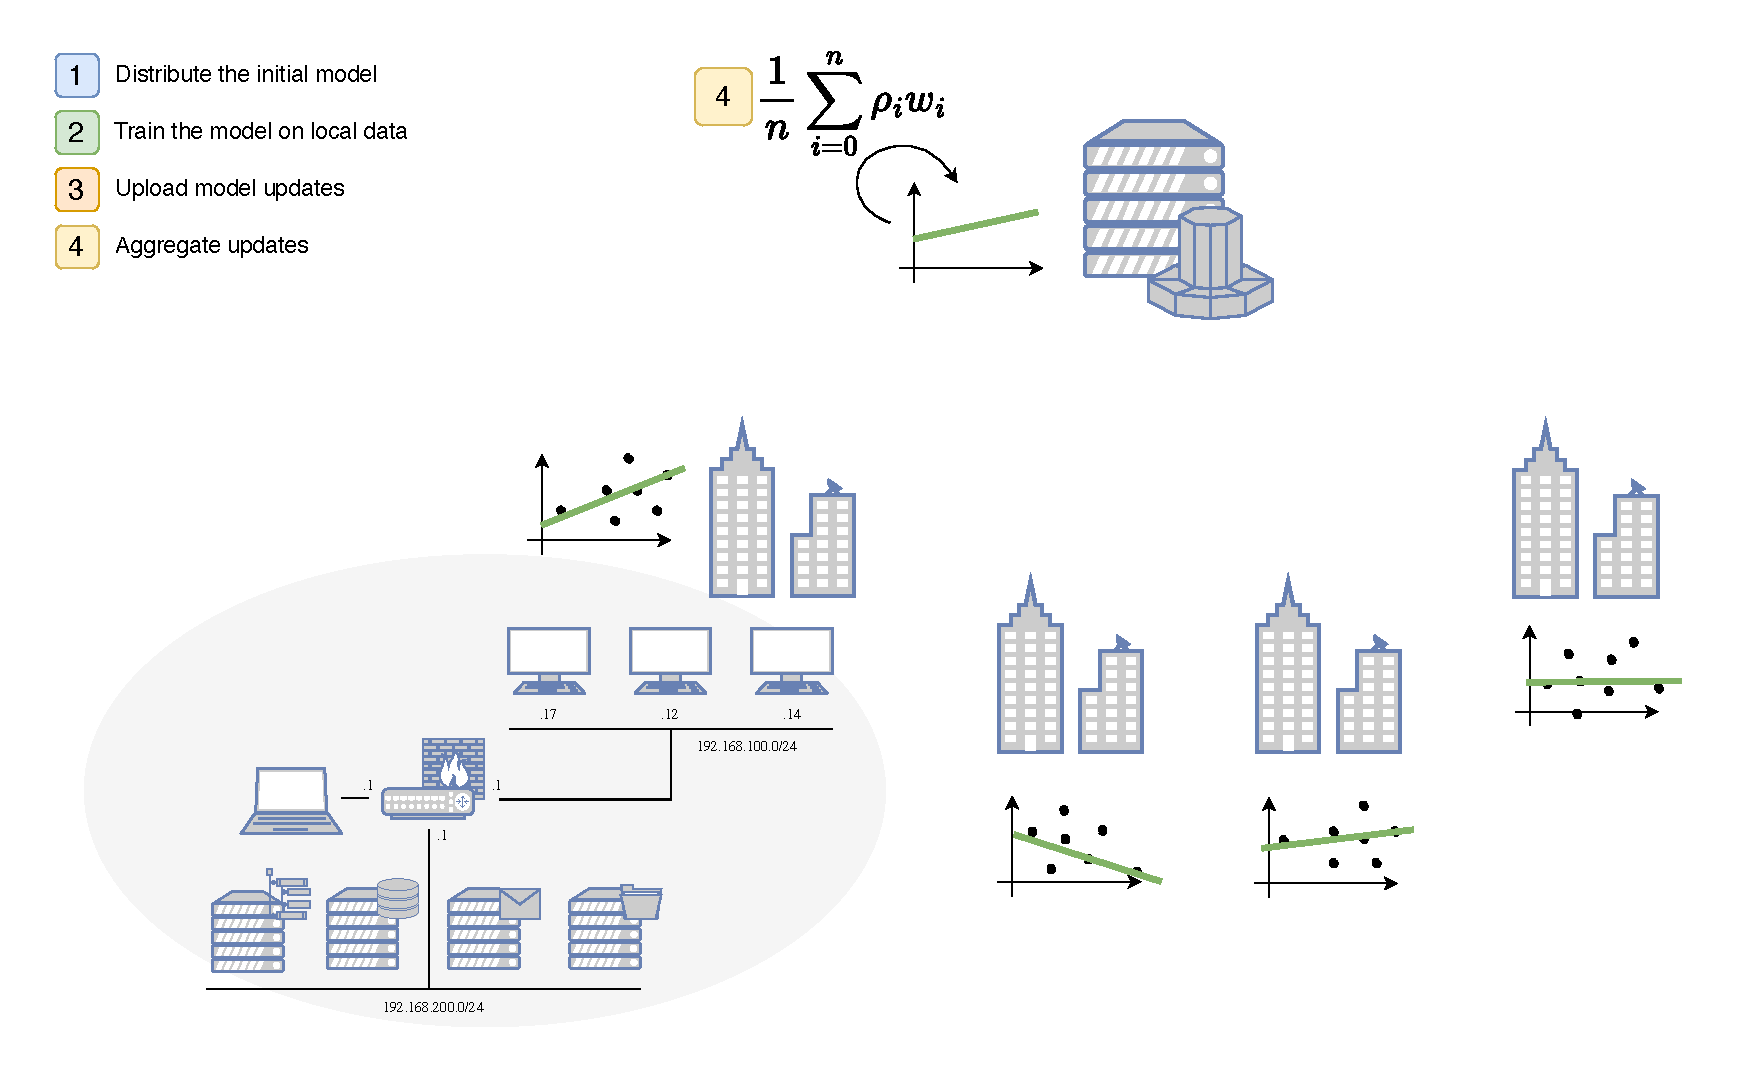
\includegraphics[width=.75\linewidth]{./figures/intro/fl/4.pdf}}%
    \only<6>{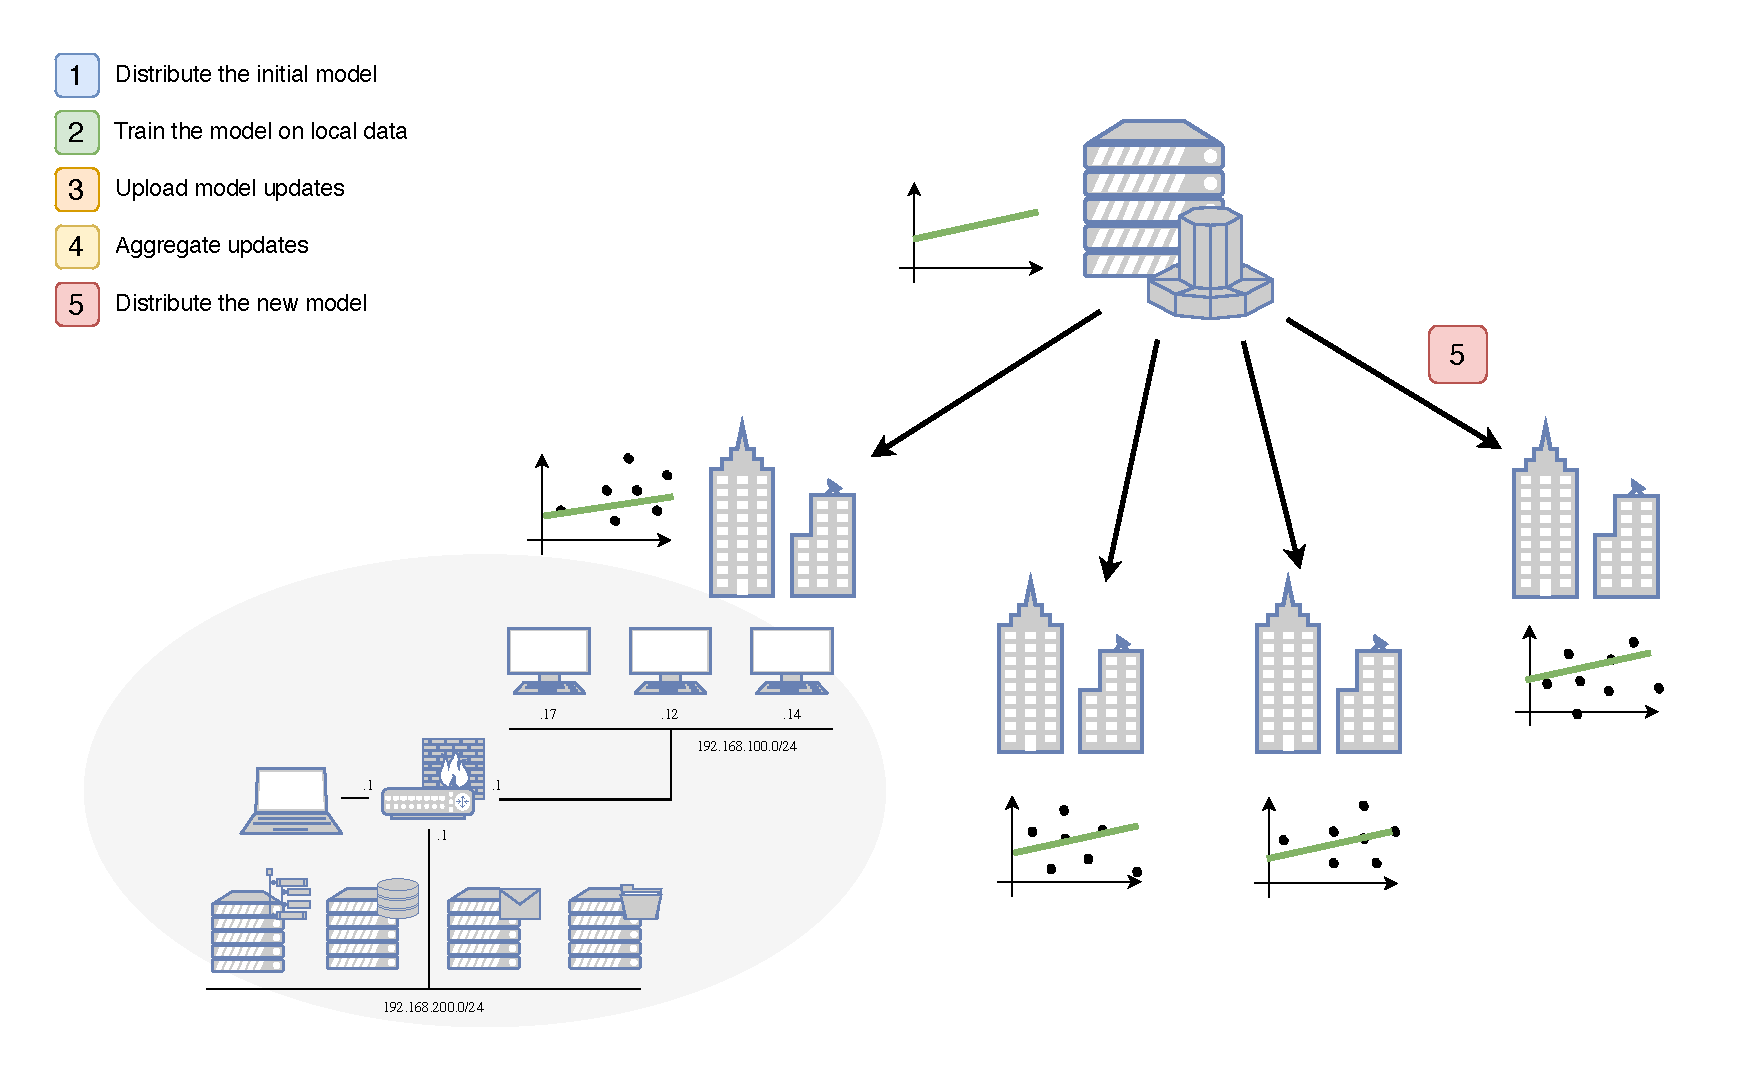
\includegraphics[width=.75\linewidth]{./figures/intro/fl/5.pdf}}%
    \only<7>{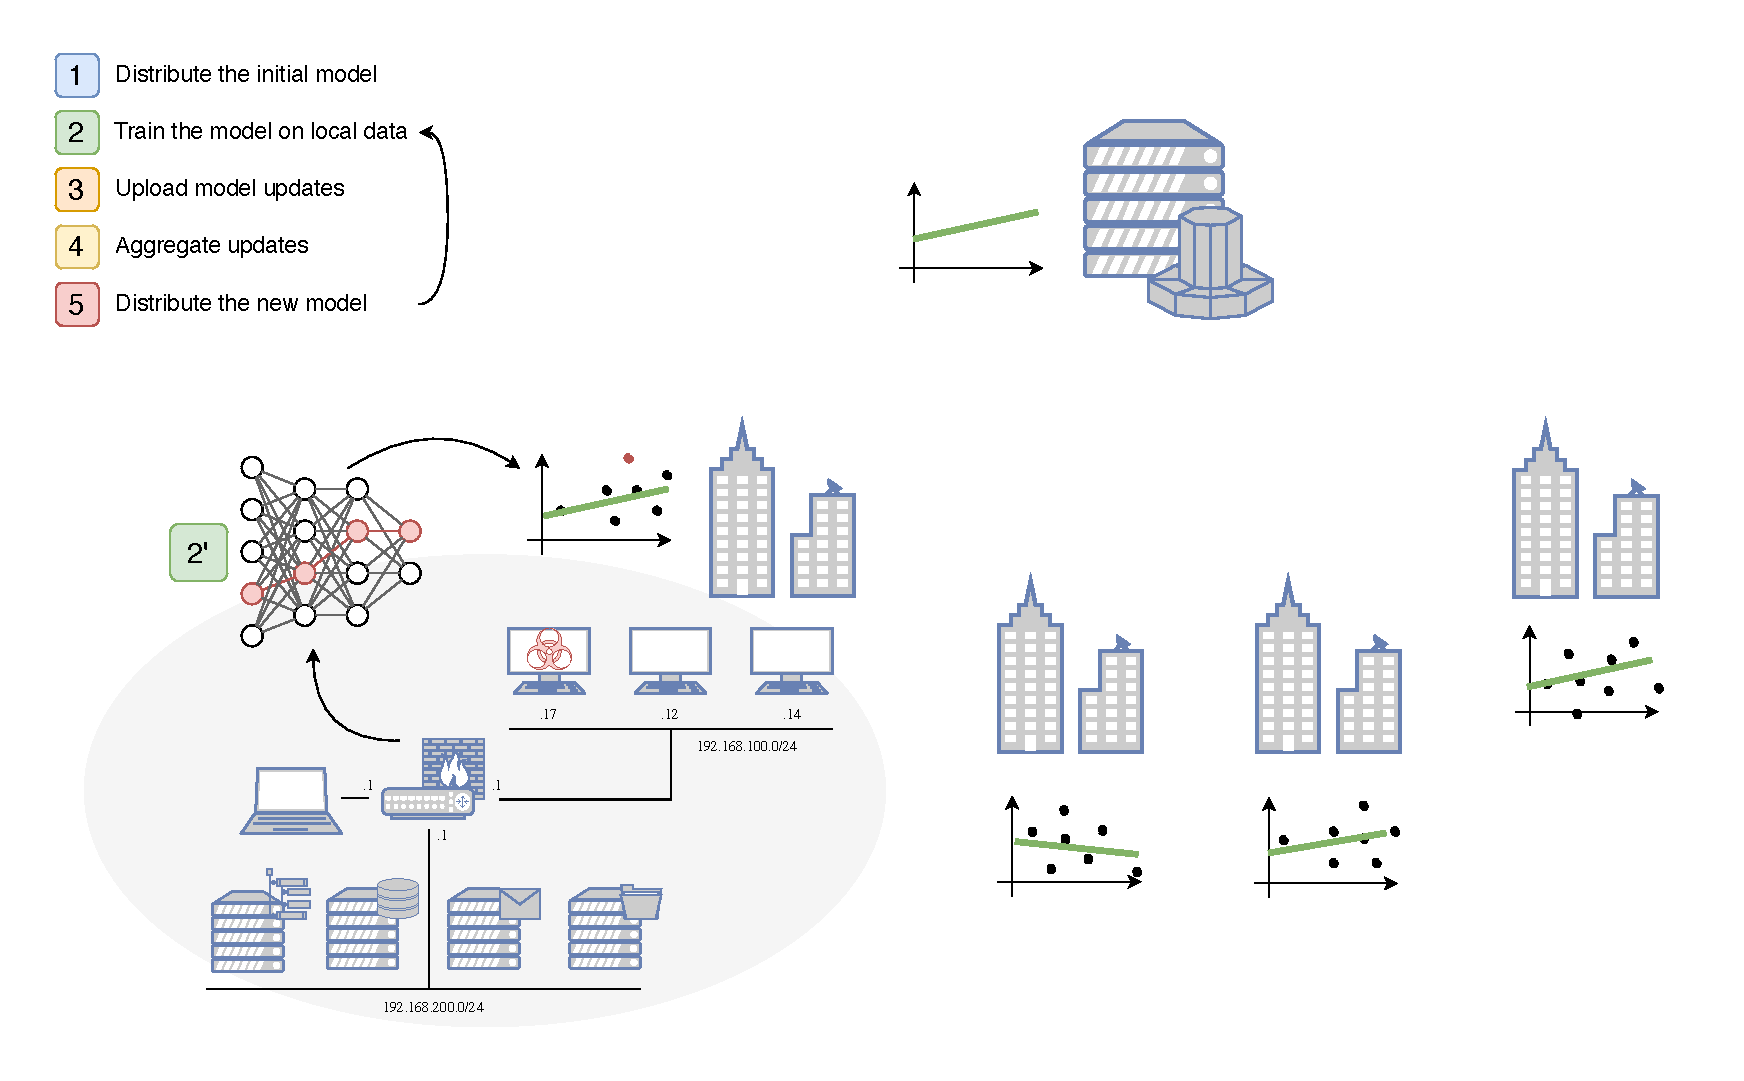
\includegraphics[width=.75\linewidth]{./figures/intro/fl/6.pdf}}%
    \caption{Typical FL workflow, applied to NIDSs.}
  \end{figure}
\end{frame}

\begin{frame}{FL for NIDSs}

  \textbf{Benefits}
  \begin{itemize}[<+->]
    \item Virtually extended dataset with Horizontal FL.
    \begin{itemize}[<1->]
      \item Better generalization.
      \item Reduced risk of overfitting or local bias.
    \end{itemize}
    

    \item Effectively share knowledge (\eg, on specific classes, instances) between participants
    \begin{itemize}[<1->]
      \item Share the knowledge about a new attack~\autocite{lavaur_icdcs_demo_2024};
      \item Improve the characterization of specific devices; \dots
    \end{itemize}

    \only<2>{\fcitefootnote{lavaur_icdcs_demo_2024}}

  \end{itemize}
\end{frame}


\end{document}
